\documentclass[10pt,a4paper,twoside,frenchb,english]{book}                % options used for 'Hoofdstuk' or 'Chapter'

%%%%%%%%%%%%%%%%%%%%%%%%%%
%% PACKAGE LOADING TIME %%
%%%%%%%%%%%%%%%%%%%%%%%%%%

%\usepackage{lscape}
\usepackage{pseudocode}
\usepackage{times}      % use Times New Roman Type 1 fonts  (redefines sfdefault,rmdefault,ttdefault)
\usepackage[utf8]{inputenc}
\usepackage[francais]{babel}
\usepackage[T1]{fontenc}

%\usepackage{pslatex}
\usepackage[times]{quotchap}   % fancy chapter beginning
\usepackage{fancyhdr}
%\usepackage[sectionbib]{chapterbib2} % bibliography per chapter
% (sectionbib -> bibliography is \section* instead of \chapter*), should come before babel chapterbib2 
%because local version is 1.9 and solves bug that header was 'References' instead of Chaptername
%\usepackage[sectionbib,numbers,sort&compress]{natbib}  %for citations a la 'Vermeulen et al.' instead of [1]
%\usepackage{tocbibind} % automatically add bibliography, list of figures, ... to table of contents
\usepackage[a4paper,verbose, asymmetric, centering]{geometry}  % better control over margins
%\usepackage[hang]{caption}     %better control over captions (sideways, font, ...)  hang -> 2nd line of caption is indented (caption2 is deprecated and beta)
\usepackage[justification=centering]{caption}     %better control over captions (sideways, font, ...)  
\usepackage{subfigure}  % with scriptsize or so, one can adapt the size
\usepackage{cite}

\usepackage{enumerate}  % to make it possible to define the numbers (A,a, ...)
\usepackage{verbatim}   % extra support for verbatim environments
\usepackage{float}      % you can define 'H' so that floats are forced to be putted 'here'
\usepackage{multirow}   % multirow{nrows}[bigstruts]{width}[fixup]{text} multirow cells
\ifx\pdftexversion\undefined
\usepackage[dvips]{graphicx}
\else
\usepackage[pdftex]{graphicx}
\fi
%\usepackage{psfrag}
\usepackage{amsmath}
\usepackage{chappg}     % page numbering (chapno-pageno), for ToC
\usepackage{url}        % for better url typesetting
\usepackage{expdlist}   % Expanded description (e.g. better alignement) -> needed for acronym_expdlist package
\usepackage{acronym_expdlist}   % for list of acronyms
\usepackage{hhline}     % generates nicer table lines (without missing pixels) + more flexible
%\usepackage{colortbl}  % for coloured columns
%\usepackage{threeparttable}     % adds the possibility to add footnotes in tables
\usepackage{afterpage}  % adds \afterpage command, which makes it possible to issue \afterpage{\clearpage} which flushes all floats after this page
%\usepackage{amsmath}    % adds extra commands, ao. \text within math environment
\usepackage{amsmath,amsfonts,amsthm}
\usepackage{marvosym}   % for Euro symbol
\usepackage{ifthen}     % ifthenelse command
%\usepackage{mathenv}	% better eqnarray
\usepackage{listings}


%%%%%%%%%%%%%%%%%
%% PAGE LAYOUT %%
%%%%%%%%%%%%%%%%%

%%%%%%%%%%%%%%%%%%%%%%%%%%%%%%%%%%%%%%%%%%%%%%%%%%%%%%%%%%%%%%%%%%%%%%
% document: page_layout_definition.tex
%
% last modified: $Id: page_layout_definition.tex,v 1.1 2005/11/18 11:49:23 bvolckae Exp $
%UPDATED ON 05/02/2014 BY SEVENOIS RUBEN TO KEEP COMPATIBILITY WITH NEWER PACKAGE VERSIONS
%
% author: Filip De Turck, Stefaan Vanhastel, Bart Duysburgh, Brecht Vermeulen, Bruno Volckaert, Steven Van den Berghe
%%%%%%%%%%%%%%%%%%%%%%%%%%%%%%%%%%%%%%%%%%%%%%%%%%%%%%%%%%%%%%%%%%%%%%

%%%%%%%%%%%%%%%%%%%%%%%%%%%%%%%%%%%%%%%%%%%%%%%%%%%%%%%%%%%%%%%%%%%%%%

%
% basic dimensions when printing the small page %
% and by using the geometry package             %

% settings Filip en Stefaan
%\geometry{bottom=4.0cm,rmargin=4.25cm,body={12.5cm,19.5cm}} % 10pt op a4
%\geometry{marginpar=0.0cm,marginparsep=0.0cm,twosideshift=0.0cm}

% new settings (according book pim which was approved by the promotors) by Bart Duysburgh
%\geometry{bottom=5.34cm,rmargin=4.5cm,body={11.5cm,18.92cm}} % 10pt op a4
%\geometry{marginpar=0.0cm,marginparsep=0.0cm,twosideshift=0.0cm}

%\geometry{body={15.5cm,18.92cm}} % 10pt op a4
\geometry{bottom=5.34cm,rmargin=4.5cm,body={11.5cm,18.92cm}} % 10pt op a4
%\geometry{twoside,marginpar=0.0cm,marginparsep=0.0cm}%,twosideshift=0.0cm}

%\geometry{bottom=2.15cm,rmargin=2.5cm,body={14.14125cm,23.6cm}} % 12pt op a4

%%%%%%%%%%%%%%%%%%%%%%%%%%%%%%%%%%%%%%%

\setlength{\textwidth}{13.5cm}
%\setlength{\textheight}{19.5cm}
%\setlength{\topmargin}{0.0cm}
%\setlength{\oddsidemargin}{0.7cm}
%\setlength{\evensidemargin}{0.7cm}
%\setlength{\marginparwidth}{0pt}
%\setlength{\marginparsep}{0pt}

%%%%%%%%%%%%%%%%%%%%%%%%%%%%%%%%%%%%%%%

\renewcommand{\topfraction}{0.8}

%%%%%%%%%%%%%%%%%%%%%%%%%%%%%%%%%%%%%%%

%%%%%%%%%%%%%%%%%%%%%%%%%%%%%%%%%%%%%%
%% change for subfigure
\renewcommand{\subfigcapskip}{0pt}
%%%%%%%%%%%%%%%%%%%%%%%%%%%%%%%%%%%%%%

%%%%%%%%%%%%%%%%%%%%%%%%%%%%%%%%%%%%%%%
% headings %

\fancypagestyle{plain}{
\fancyhf{}
\renewcommand{\headrulewidth}{0pt}
\renewcommand{\footrulewidth}{0pt}}

\pagestyle{fancy}
\fancyhf{} %clear all header and footer fields
\addtolength{\headwidth}{\marginparsep}
\addtolength{\headwidth}{\marginparwidth}

%\renewcommand{\chaptermark}[1]{\markboth{\chaptername\ \thechapter. \ #1}{}}

\renewcommand{\chaptermark}[1]{\markboth{#1}{}}
%\renewcommand{\sectionmark}[1]{\markright{\thesection\ #1}}

%\newcommand\fdtsvrightmarktmp{{\scshape\small Chapter }}
%\newcommand\fdtsvrightmark{{\scshape\small{Acknowledgment}}}
%\newcommand\fdtsvleftmark{{\scshape\small{Dankwoord}}}

\newcommand\oddpageleftmark{}
\newcommand\evenpagerightmark{}

%\fancyhead[LE,RO]{\itshape\bfseries\small\thepage}
%\fancyhead[LO]{\itshape\bfseries\small\leftmark}
%\fancyhead[RE]{\itshape\bfseries\small\rightmark}
\fancyhead[LE,RO]{\small\thepage}
\fancyhead[LO]{\oddpageleftmark}
\fancyhead[RE]{\evenpagerightmark}
%\fancyfoot[C]{\itshape\bfseries\footnotesize \chaptername\ \thechapter}

%%%%%%%%%%%%%%%%%%%%%%%%%%%%%%%%%%%%%%%%%%%%%%%%%%%%


%%%%%%%%%%%%%%%%%%%%%%%%%%%%%%%%%%%%%%%%%%%%%%%%%%%%
% depth of numbering and depth of table of contents %

\setcounter{tocdepth}{3} % titels tot en met niveau subsubsection worden in table of contents opgenomen
\setcounter{secnumdepth}{3} % tot en met niveau subsubsection wordt er genummerd
%%%%%%%%%%%%%%%%%%%%%%%%%%%%%%%%%%%%%%%%%%%%%%%%%%%



%%%%%%%%%%%%%%%%%%%%%%%%%%%%%%%%%%%%%%%%%%%%%%%%%%%
%%%%% Definition for Big letter at the beginning of a paragraph %%
\def\PARstart#1#2{\begingroup\def\par{\endgraf\endgroup\lineskiplimit=0pt}
    \setbox2=\hbox{\uppercase{#2} }\newdimen\tmpht \tmpht \ht2
    \advance\tmpht by \baselineskip\font\hhuge=cmr10 at \tmpht
    \setbox1=\hbox{{\hhuge #1}}
    \count7=\tmpht \count8=\ht1\divide\count8 by 1000 \divide\count7 by\count8
    \tmpht=.001\tmpht\multiply\tmpht by \count7\font\hhuge=cmr10 at \tmpht
    \setbox1=\hbox{{\hhuge #1}} \noindent \hangindent1.05\wd1
    \hangafter=-2 {\hskip-\hangindent \lower1\ht1\hbox{\raise1.0\ht2\copy1}%
    \kern-0\wd1}\copy2\lineskiplimit=-1000pt}
%%%%%%%%%%%%%%%%%%%%%%%%%%%%%%%%%%%%


%%%%%%%%%%%%%%%%%%%%%%%%%%%%%%%%%%%%%%%%%%%%%%%%%%%%
%%% Nog een paar andere zaken  %%%%
%% om een cross-ref naar een voetnoot te kunnen maken definier ik \usefn %%
\newcommand{\usefn}[1]{\mbox{\textsuperscript{\normalfont#1}}}

%\setlength{\captionindent}{1cm}
\renewcommand{\captionfont}{\small \itshape \mdseries \rmfamily}
\renewcommand{\subcapsize}{\footnotesize \itshape \mdseries \rmfamily}

\AtBeginDocument{%
%   \renewcommand{\figurename}{Fig.}%
%   \renewcommand{\tablename}{TABLE}%
   \renewcommand{\tablename}{Table}
  % \renewcommand{\bibname}{References}%
}

%%%%%%%%%%%%%%%%%%%%%%%%%%%%%%%%%%%%%%%%%%%%%%%%%%%



%%%%%%%%%%%%%%%%%
%% HYPHENATION %%
%%%%%%%%%%%%%%%%%

%%%%%%%%%%%%%%%%%%%%
%%  START BOOK    %%
%%%%%%%%%%%%%%%%%%%%

\begin{document}
\graphicspath{{fig/}}
\restylefloat{figure}
\restylefloat{table}

%%   FRONT PAGE       %%
%%%%%%%%%%%%%%%%%%%%%%%%
% 
 \thispagestyle{empty}   % no headings for this page
% 
% % Header
 \noindent
 \begin{minipage}{3cm}%
   \includegraphics*[width=2cm]{UGentlogo}% logo ugent
 \end{minipage}\hfill
 \begin{minipage}{8cm}
 \raggedleft
 \textsf{Ecole Centrale Paris\\
Université Paris-Saclay}
 \end{minipage}
% 
% % Title
\bigskip
   \begin{flushleft}
     \Large \textsf{Production de gaz de synthèse par oxydation partielle à haute pression. \\
Conception et dimensionnement de technologies de combustion.}

   \end{flushleft}
 \hrule
% 
 \bigskip
   \LARGE\noindent \textsf{Arthur Degenève} \hfill
 \bigskip
% 
% % Front Figure
% %\bigskip
% %\begin{figure}[htb]%
% %  \centering%
% %  \includegraphics*[width=\textwidth]{figFront}%
% %\end{figure}%
% %\normalsize
% 
% \bigskip
% \begin{figure}[h!]%
%   \centering%
%   \includegraphics*[height=10cm, keepaspectratio, clip]{figFront}%
% \end{figure}%
 \normalsize
% 
% % Footer
 \vfill
 \begin{minipage}{2.0cm}%
     \includegraphics*[width=2.0cm]{intec}%       % intec logo
 \end{minipage}\hfill
 \begin{minipage}{9cm}
 \raggedleft
 \textsf{Arthur Degenève \\
 Stage master recherche M2: }
 \end{minipage}


%% INFORMATION PAGE     %%
%%%%%%%%%%%%%%%%%%%%%%%%%%

\clearpage{\pagestyle{empty}\cleardoublepage}


\clearpage{\pagestyle{empty}\cleardoublepage}


%% ACKNOWLEDGMENT   %%
%%%%%%%%%%%%%%%%%%%%%%%


\hyphenation{bu-reau-ge-no-ten}
\frontmatter
\chapter{}
\vspace{0.35in}

\selectlanguage{english}

\clearpage{\pagestyle{empty}\cleardoublepage}

%%   TOC, LIST OF FIGURES, LIST OF TABLES, ACRONYMS     %%
%%%%%%%%%%%%%%%%%%%%%%%%%%%%%%%%%%%%%%%%%%%%%%%%%%%%%%%%%%

\renewcommand{\contentsname}{Table of Contents} % original name = Contents

\tableofcontents
\clearpage{\pagestyle{empty}\cleardoublepage}

\listoffigures
\clearpage{\pagestyle{empty}\cleardoublepage}

\listoftables
\clearpage{\pagestyle{empty}\cleardoublepage}

% List of Acronyms
%%%%%%%%%%%%%%%%%%%%%%%%%%%%%%%%%%%%%%%%%%%%%%%%%%%%%%%%%%%%%%%%%%%%%

\chapter*{List of Acronyms}
%     \@mkboth{\MakeUppercase List of Acronyms}%
%              {\MakeUppercase List of Acronyms}%

%\begin{center}
%\textbf{\Large List of Acronyms}
%\end{center}
\textbf{\newline\newline\Large A} \newline
\begin{acronym_expdlist}
\acro{ACE}{Adaptive Communication Environment}
\end{acronym_expdlist}




\clearpage      % clear the current page
\thispagestyle{empty}   % prevent header on this (empty -> next line) page
\mbox{}         % to insert a not empty page, so that there is min. 1 blank page before next chapter
\clearpage{\pagestyle{empty}\cleardoublepage}   % clear the current page and start on the right side

%\renewcommand{\tablename}{Table}

%\renewcommand{\bibname}{References}     % instead of Bibliography
%\renewcommand\citeform{\thechapter.}
%\addcontentsline{toc}{section}{\listfigurename}   % not really sure


%% THE BOOK ITSELF   %%
%%%%%%%%%%%%%%%%%%%%%%%
\mainmatter     % related to chappg numbering
\selectlanguage{english}

\newcommand\fdtsvrightmarktmp{{\scshape\small Chapter }}
\renewcommand\evenpagerightmark{{\scshape\small\chaptername\ \thechapter}}
\renewcommand\oddpageleftmark{{\scshape\small\leftmark}}

%\addtolength{\headwidth}{\marginparsep}
%\addtolength{\headwidth}{\marginparwidth}

%\newcommand{\tm}[1]{$\mbox{#1}^{\mbox{\emph{\scriptsize TM}}}$}

\baselineskip 13.0pt
\graphicspath{{chapt_dutch/}{intro/}{chapt2/}{chapt3/}{chapt4/}{chapt5/}}

% Header
\renewcommand\evenpagerightmark{{\scshape\small Appendix A}}
\renewcommand\oddpageleftmark{{\scshape\small Grid Computing: The Next Network Challenge!}}

%\renewcommand{\bibname}{References}

\hyphenation{}

\chapter[Appendice 1]%
{Appendice 1}
\label{app1}


\emph{
abstract
}

\section{Introduction}
Start text here...



\clearpage{\pagestyle{empty}\cleardoublepage}



% Header
\renewcommand\evenpagerightmark{{\scshape\small Internship overview}}
\renewcommand\oddpageleftmark{{\scshape\small Chapter 2}}

\renewcommand{\bibname}{References}

\hyphenation{}

\chapter[Premières réflexions]%
{Premières réflexions}
\label{premieres_reflexions}

\section{Besoins industriels d'Air Liquide}
Aujourd'hui, les règles de dimensionnement des fours ATR et POX sont mal maîtrisées. Développée par Lurgi, l'ingénierie des fours ATR/POX d'Air liquide n'est pas encore prédictive et la conception manque d'outils pour dimensionner les brûleurs. Air Liquide veut donc davantage maîtriser les process dans le but de :
\begin{itemize}
\item Augmenter la production en sortie de gaz
\item Maîtriser davantage les rejets
\item Obtenir des syngazs de meilleurs qualités (?)
\end{itemize}

Dans ce but, un pilote a été construit en 2004 à Freiberg, reproduisant les conditions des fours industriels. Ce pilote peut fonctionner en plusieurs configurations, notamment ATR. Il dispose de quelques diagnostics, notamment images de la flamme et bilans de masse entrée/sortie. De nombreux tests ont été conduits sur ce brûleur et ces données sont le point de départ du stage.

A travers ce stage, Air Liquide désire :
\begin{itemize}
\item Obtenir des règles de dimensionnement pour les brûleur ATR : lois d'échelles par des nombres adimensionnés adaptés, justifier des choix technologiques
\item Comprendre le comportement des flammes et les mécanismes responsables
\item Donner de la visibilité au numérique, qui manque aujourd'hui cruellement de données expérimentales pour justifier les modèles
\item Dans les paramètres observés par Air Liquide, la forme de la flamme est primordiale, on cherche à bien maîtriser la température au niveau de l'entrée du catalyseur
\end{itemize}

\subsection{Les brûleurs utilisés}
Le pilote HPPOX peut se mettre en mode ATR et son brûleur porte la dénomination ATR-30norm, ce n'est pas le même brûleur que les brûleurs de production des fours ATR industriels. De part la taille déjà, en revanche, on garde des rapports de géométries similaires, et notamment les angles des aubes à 30 et 20.

\subsection{L'ATR au sein de la R\&D aux loges}

Peu de travaux faits sur les ATR, et la majorité concerne l'équipe MathApp. Les volumes d'ATR vendus sont faibles mais sont toujours des investissements conséquents. Air Liquide s'intéresse de nouveaux aux ATR depuis le rachat de Lurgi mais l'appropriation et la remise en questions de la conception des ATR nécessite du temps.

\section{Déroulé et plans du stage}
\begin{enumerate}
\item Travail de bibliographie sur les fours ATR et l'influence du nombre de swirl
\item Identification des paramètres qui pilotent : Re, Swirl1, Swirl2, rapport impulsion
\item Etude et dimensionnement des brûleurs à utiliser et de leur conception
\begin{itemize}
\item Fabrication industrielle (cas le plus simple et le plus rapide)
\item Faisabilité du prototypage rapide (le cas échéant)
\end{itemize}
\item Pour chaque brûleur :
\begin{itemize}
\item Diagnostics expérimentaux
\item Régimes de flammes
\item Comparaison avec le pilot HPPOX
\end{itemize}
\end{enumerate}

\subsection{Les intuitions initiales Air Liquide}

Au 1er ordre, c'est la diffusion turbulente qui pilote.

Puisqu'on ne peut pas reproduire Freiberg au labo, il faut respecter l'ordre des échelles pour se rapprocher des mécanismes, en particulier regarder l'évolution dans le diagramme Poisot Veynante. On respecterait cette ordre en conservant :
\begin{itemize}
\item Nombres de swirls équivalents
\item Même rapports d'impulsions
\item Même géométrie
\item Même vitesse
\end{itemize}
Du coup avec des valeurs différentes pour :
\begin{itemize}
\item la pression
\item la richesse
\item le nombre de Reynolds
\end{itemize}
Pour ce qui est de la pression et de la densité, on estime que les mécanismes responsable est davantage le gradient de densité, gradient que l'on veut conserver par le biais des températures (à vérifier).

Concernant la richesse, elle est primordiale dans en combustion prémélangée mais nettement moins en diffusion, dans le mesure ou la flamme se fait en particulier à la stoechiométrie. 

En revanche, il n'y aura pas de réaction de réformage car le méthane sera en défaut. Les diagnostics à comparer avec Freiberg seront donc uniquement des visualisations de flammes. Les canaux seront également inversés entre combustibles et oxydants

\section{The scientific strategy of the internship}

\subsection{The mechanisms driving the topology of the flame}

It must be defined whether the topology of the flame depends on the kinetic or the description of the mixture (diffusion and turbulence). Here are the pros and cons :
\paragraph{Turbulence is driving the flame}
\begin{itemize}

\item According to Veynante - Darabiha, the diffusion flame are mostly driven by the turbulence, and the kinetic can considered as infinitely fast. The argument is not fully verified of course here, this is the purpose of the internship of Ru to study the influence of the kinetic on the topology of the flame
\item This is also an the presumption of Bernard Labegorre and Air Liquide to consider that the turbulent diffusion is the 1st parameter to have an influence on the flame
\item When taking into account a better mixture with LES computation, the topology of the flame is closer to the one is HPPOX

\end{itemize}
\paragraph{Kinetic is driving the flame}
\begin{itemize}
\item The article (\# ref Milosavljevic, V. D., Taylor, A. M. K. P., and
Whitelaw, J. H., Imperial College, Department of
Mechanical Engineering report FS/87/35, (1987).) enhances that a high Reynolds or Swirl number can reach the maximum kinetic velocity so that the kinetic will limit the combustion
\item When using kinetic schemes instead of infinite kinetic, the flame is shorter
\end{itemize}

\subsection{Cooperation with Ru}

Ru and I have two approaches than can be gathered. Even if it is not the only task, we both have to reproduce the results of Freiberg burner, me experimentally and Ru through simulation. It the goal is achieved, implying that we have similar flame topologies, flame length and so on, there are benefits to work together :
\begin{itemize}
\item To my concern, if Ru and I have the same topology of flame, then assuming certain hypothesis, I can find back the velocity field through the simulations of Ru
\item To Ru's concern, we can try different experimental configuration to assess the reliability of her simulation
\end{itemize}

\subsection{Les paramètres expérimentaux}
\paragraph{Nombre de swirl}
Le dispositif sera toujours à aubes fixes, on modifiera dans le nouveau bruleur pilote les nombres de swirls en modifiant la répartition des débits axiaux/tangentiels.
Si on voit que c'est un paramètre de premier ordre, on pourra alors proposer de modifier les swirls sur les bruleurs ATR30-norm, ce qui n'a jamais été fait avant.
\paragraph{Nombre de Reynolds}
Sera limité par la capacité du brûleur, on pourra le baisser légèrement mais ce ne sera vraisemblablement pas un paramètre de premier ordre
\paragraph{rapport d'impulsions}
Avec des outils d'analyses dimensionnelles type Vaschi Buckingham, on fera peut-être apparaître ce paramètre. Voir son influence dans la littérature.
\paragraph{Rapport de dillution à l'azote}
Dans la mesure où il n'y aura pas de réactions de reformage, la vapeur d'eau n'intervient pas et on utilisera de l'azote comme diluant. Le rapport de dilution pourra être intéressant pour diminuer la part de méthane, ainsi diminuer la puissance du bruleur tout en conservant les memes vitesses qu'a Freiberg. Ainsi, c'est pour l'instant un paramètre libre qu'on pourra fitter pour s'accorder à la flamme de Freiberg.
\paragraph{Qarl number}

\clearpage


\clearpage{\pagestyle{empty}\cleardoublepage}

\renewcommand\evenpagerightmark{{\scshape\small Scan of the literature}}
\chapter[Scan of the literature]%
{Revue de Biblio}
\label{revue_de_biblio}
\section{Scale-up et lois d'échelles}

\subsection{Le scale-up peut marcher en éloignant le débit transverse}
\cite{shigeru_azuhata_scale-up_study_of_gas_composition.pdf_1986}
Cet article indique que le scale-up peut-être fait si on fait attention au mélange transverse de l'oxydant dans le fuel. Il recommande par exemple d'éloigner fortement l'arrivée d'air transverse comme il le fait avec son brûleur B. 

Comme explication, l'allumage dépend de la pénétration de l'oxydant dans le fuel, à même vitesse un petit brûleur serait favorisé car son diamètre est plus petit (?)

Mais on pourrait également prendre gare à conserver dans le brûleur ce mécanisme.

\subsection{Scale-up with detonation}

\cite{fig_experimental_2016} this article, scale-up has been experimentally studied with detonation flames : with tubes from 5cm to 71cm, the maximum burning velocity has been fitted with a power fit, which has permitted to forecast the burning velocity for the bigger pipe (71cm) before the experimental setup was finished. The accuracy of the prediction is very good. The power of the fit is not given.

But no explanations of the scale mechanisms is given in this article.
\section{Influence of the Reynolds number}

Article \cite{milosavljevic_influence_1990}  says that increasing the Reynolds number shortens the flame length. If it is due to Reynolds number, it can be bad for the internship, otherwise if it depends more on the bulk velocity, then since we will use the same velocities as the HPPOX, it should be ok. 

Internal Air Liquide (\# ref Freiberg) report showed that between 30 and 40 bar, the flame was the same (length, topology, width...).  Here, pressure mainly modifies the Reynolds number.


\section{Influence of the Swirl number}

\subsection{Recirculation}

Recirculation is generally not observed for swirl numbers below 0.4, so most swirl-stabilized burners are designed for swirl numbers greater than 0.6.

\subsection{Solid body rotation}

On a normalement un solid body rotation pour $r<R/2$ \cite{toh_axial_2010} , cela peut monter plus haut si le swirl augmente \cite{durox_flame_2013}.

\subsection{Flame topology}

between two kinds of burners, the flame topologies can vary a lot, even with the same swirl number. It is particularly the case depending on axial/radial swirl. For example, the shapes are very different between \cite{paul_jourdaine_nom_effect_2016} and \cite{durox_flame_2013}.

From an analysis point of view, it clearly shows that the swirl number is not the only adimensional quantity to describe a swirling flow. The quarl angle is another one, but even if with a quarl angle of $0^\circ$, we need another one to describe why we find a peak in Paul Jourdaine's profile and not the ones of Durox.

\subsection{As the increasing of Reynolds narrows the lean limit, the increasing Swirl may narrows the lean limit as well}

When the bulk velocity increases (equivalent to the Reynolds number), the kinetics reaches its limits so that it increases the lean limit (the rise in the Re is not followed by a rise in the kinetics (which has reached its maximum) so that the flame blows out.

It may be the same case with Swirl number \cite{milosavljevic_influence_1990}. Since the rise in Swirl implies a rise in the tangential velocity, once the maximum kinetic velocity is reached, the rise in the Swirl number can only narrows the lean limits. But it does not explain the bulges of the articles in Fig 3 (there are some discrete values of Swirl where the lean limit is very high, and the flame very stable).

\subsection{Central recirculation zone (CRZ) is independent of S}
This is not the case with the flame length! 

L'article\cite{milosavljevic_influence_1990}  fait varier grandement le nombre de swirls, le quarl et le type de brûleurs pour en tirer ces conclusions, for a given equivalence ratio:
\begin{itemize}
\item The recirculation length is independant of the Swirl number, of the bulk injection (equivalent to Reynolds) and of a second order with the type of nozzle used
\item Strongly depends on the quarl number (CRZ increases with the quarl)
\end{itemize}


\subsection{PVC frequency is a linear function of Re}
\cite{martinelli_experimental_2007} According to that article, it is admitted today that the precessing frequency of the PVC is a linear function of the Reynolds number, assuming swirl number S =cste.

\subsection{Using the same adiabatic flame temperature in order to compare different dilutions}
Paul Jourdaine \cite{paul_jourdaine_nom_effect_2016} showed that the topologies of flame are the same between C02 and N2 if the adiabatic flame temperature is respected. The dilution is consequently of second order, this is perfect for the purpose of the internship since it is planned to use another diluent than the PPOX. This is a very powerful results, and the results are still verified if the Swirl number or the quarl number vary.

\section{The quarl angle}

"Ouvreau" in french, the quarl is a piece used in the burner in order to protect the flame from the edge of the burner. One can give a certain angle and \cite{paul_jourdaine_nom_effect_2016} studied the influence of quarl number on a premixed flame. From $0^\circ $ to $45^\circ $, the increase of the quarl number decreases the flame length, and flatten the shape of the flame. Above all, the use of the quarl number is another degree of freedom to shape the flame according to the industrial needs.

According to\cite{milosavljevic_influence_1990}, the CRZ increases as the quarl angles increases.	

\section{Influence of S/C ratio}

According to \# ref Freiberg the flame and the width increases as S/C ratio decreases.

\section{The calculation of the Swirl number}

The only way to be reliable on a Swirl number is to measure it with integration with LDV profile. Since it is not affordable, geometrical approach is necessary to give a 1st value, which can be as false as 100\% error according to the literature.

To do so, the only way is to make assumption on the shape of the velocity field. The calculation of the geometrical swirl number is then only a question of assumption on the shape of the velocity field.

\section{The shape of the velocity field}

If the swirl number is not so important, we can use the results of \cite{durox_flame_2013} to make assumptions, they are very well documented and such shapes of velocity field are quite commonly found in the literature. 

\subsubsection{The Axial Velocity}

If the Swirl number is not high, assuming a constant axial velocity is false but remains the best option and can be quite accurate for low swirl numbers. From now, let us assume $u_{z}=cste$.

\subsubsection{The Tangential velocity}

Three main simple velocity field can be assumed :
\begin{enumerate}
\item $u_{\theta}=cste$ this is currently used but unreliable in the center of the flow, where a discontinuity cannot be possible
\item Solid body rotation : $u_{\theta}=\Omega r$ this is quite almost always true in the center of the flow, and sometimes in the overall flow. But, most of the time, it is completely unreliable when $r \sim R$ 
\item Free vortex flow and conservation of the tangential momentum : $u_{\theta} \cdot r=cste$ This is almost always true near the walls, but unreliable in the center of the flow
\end{enumerate}

\paragraph{Navier-Stokes} I chose to use Navier Stokes cylindrical equations of the tangential velocity to confirm these assumptions. Here are the simplifications :
\begin{itemize}
\item Incompressible
\item independent from $\theta$,$z$ and time $t$, only depends on $r$ coordinate (established flow in a cylinder)
\end{itemize}
Hence, Naviers-Stokes simplifies in :

$\frac{1}{r}\frac{\partial }{\partial r}(r \cdot \frac{\partial u_{\theta(r)}}{\partial r})=\frac{u_{\theta(r)}}{r^2}$ 

Without resolving it, one can see that $u_{\theta}=\Omega r$ and $u_{\theta} \cdot r=cste$ are two particular solutions of the equations. Consequently, in most of the cases, a combination of Solid body rotation and Free vortex flow can well picture the behavior of the swirl, non forgetting that the wall viscosity will eventually drive the tangential velocity to 0 (no matter the assumption on the tangential velocity).

Further investigations will me made to explore if one can fully describe a tangential flow with the following shape : $u_{\theta}=\epsilon_{inner}(r) \Omega r + \epsilon_{outer}(r) \frac{G}{r}$ where $\Omega$ and $G$ are two unknown, and $\epsilon$ the Kronecker symbol. In the center of the vortex, the velocity could be a solid body rotation, and from a certain distance, a free vortex flow.

Nevertheless, we can observe the assumptions in the literature to see that a lot of publications calculates Swirl number without paying enough attention on the shape of the velocity field, and then deplores disparities with the result.

If $u_{\theta}=\Omega r$, then $S=1/2 \frac{u_{\theta}}{u_{z}}$ , and if $u_{\theta}=cste$, then $S=2/3 \frac{u_{\theta}}{u_{z}}$ .

\subsubsection{In case of an axial swirler}
There are two possibilities, listed in the table  :

\begin{tabular}{ l | c | r }
  \hline			
 blade & blade angle depending on $r$ & fixed blade angle \\
  burner & ATR 30norm Freiberg  & Industrial burner \\
  tangential profile & $u_{\theta}(r)=r\Omega$ & $u_{\theta}=cste$ \\
geometrical swirl &  assuming that $\vec{velocity}$ remains parallel to the blade, $S=\frac{1}{2}tan(\alpha(R))$& $S=\frac{2}{3}tan(\alpha)$ \\
  \hline  
\end{tabular}

\subsubsection{With a radial swirler}

\cite{durox_flame_2013} This article tackles the difficulties in determining with accuracy the Swirl number. One can find in the literature many formulas, but each case being different, the only way to know the Swirl number is to measure it (with LDV?). The articles criticizes the fact that many publications does not take care of the accuracy of the swirl number, so that they can be overestimated or underestimated. Depending on the formulas one chooses, there can be error of 100\%. The article study different formulas in a radial swirler, the selected ones at the end are :

\begin{itemize}
\item $S=\frac{1}{4} \frac{R}{L} tan(\alpha)$ where $R$ is the radius of the swirler and $L$ the height of the radial injection. In this formula, one uses the hypothesis of a solid body rotation $u_{\theta}(r)=\Omega r$ and can be easily demonstrated.
\item The other ones $S=0.75\frac{\bar{u_{\theta}}}{\bar{u_{z}}}$ comes from a fit and is very accurate but recquires to know $\bar{u_{\theta}}$
\end{itemize}

But is seems that the common formula from many publications (ref T.C. Claypole, N. Syred, Proc. Combust. Inst. 18 (1981) 81–89. and ref Y. Zhang, D. Shimokuri, Y. Mukae, S. Ishizuka, JSME Int. J. Ser. B 48 (4) (2005)
830–838) : $S=\frac{\pi D D_{0}}{4A_{t}}$. According to my calculation, and to the article (ref T.C. Claypole, N. Syred, Proc. Combust. Inst. 18 (1981) 81–89.), this formula comes from $S=\frac{u_{\theta}(R)u_{z}R^2}{R \cdot u_{z}^2 \cdot R}$ Which is the swirl number without the integral. It is very surprising, and the article \cite{durox_flame_2013} finds that this number is two time larger than the measurements (which would be completely corrected if it would have taken $S=1/2 \frac{u_{\theta}}{u_{z}}=\frac{\pi D D_{0}}{8A_{t}} $, corresponding to a solid body rotation in the center and a free wall vortex near the wall


\subsubsection{With an axial swirler}

The article\cite{palies_combined_2010}  uses an axial swirler and shows the difficulty of calculating a swirl number, a very interesting table compares among different publications the number of swirl, its calculations and the formulas used to compute it. Its own formula to calculate the swirl number is :$S=2/3 tan(\theta)$, and gives 100\% of inacuracy when compared to the integration of LDV profile.

\subsubsection{The strategy for the internship}

Hence, for the purpose of the internship, assuming that LDV is unreachable in Calhory furnace,  here are 3 possibilities to overcome the situation :
\begin{enumerate}
\item With a literary review, try to choose a similar burner to approach the swirl number. Or choose it arbitrarily, knowing that it would be false, but only taking into account it relatively
\item Simulating it on Fluent, with non reacting flow. The difficulty will be to create the geometry of the burner, which is very complicated
\item Use another metric to observe something else on the burner to guess the Swirl number (only possible if scale-up rules are found, or reliable behavior rules of the swirl number)
\end{enumerate}

The main problem is that the rules to compute the swirl number will first depend on the geometry of the burner. One can identify three kinds of swirler : 
\begin{enumerate}
\item the radial swirler : \cite{durox_flame_2013}, the burner with axial and tangential injections
\item the axial swirler : it is the case of the burner ATR-30
\item a mix of the two \cite{paul_jourdaine_nom_effect_2016} as it is the case in OXYTEC, or the pilot we want to build.
\end{enumerate}

To me, the determination of the swirl number must be the most accurate possible. At least, we must fully understand the perimeter of the calculation of the swirl number , these are the very important reasons why I focused on that specific matter :
\begin{enumerate}
\item The whole purpose of the internship is to show that turbulent diffusion is the first parameter who drives the topology of the flame. The industrial parameter we can change is the swirl number through the geometry of the burner. Hence, one cannot neglet the accuracy of the very parameter whose importance is to be proven on the behaviour of the flame.
\item Since we want to prove that pressure and equivalence ratio matter less than swirl and turbulent diffusion, let's be accurate on the swirl geometry!
\item The litterature can give us qui accurate topology of flames according to the swirl number. For instance, one knows that the CRZ is going to appear for S bigger than 0.4-0.6 We cannot content ourself with 100\% inacuray on the swirl number
\item We have two swirl numbers
\item The quality publications check the accuracy of the chosen formula by measuring with PIV/LDV the velocity distribution at the outlet of the burner in order to intergrate them and calculate the quite accurate swirl number. This is not possible in this internship, since we cannot use advanced optical diagnosis.
\end{enumerate}



 





\renewcommand\evenpagerightmark{{\scshape\small Scale-up}}
\chapter[Scale-up]%
{Scale-up}
\label{Scale-up}

\section{Analysis of a non reactive flow in a basic case}

\begin{figure}[!h]
  \centering
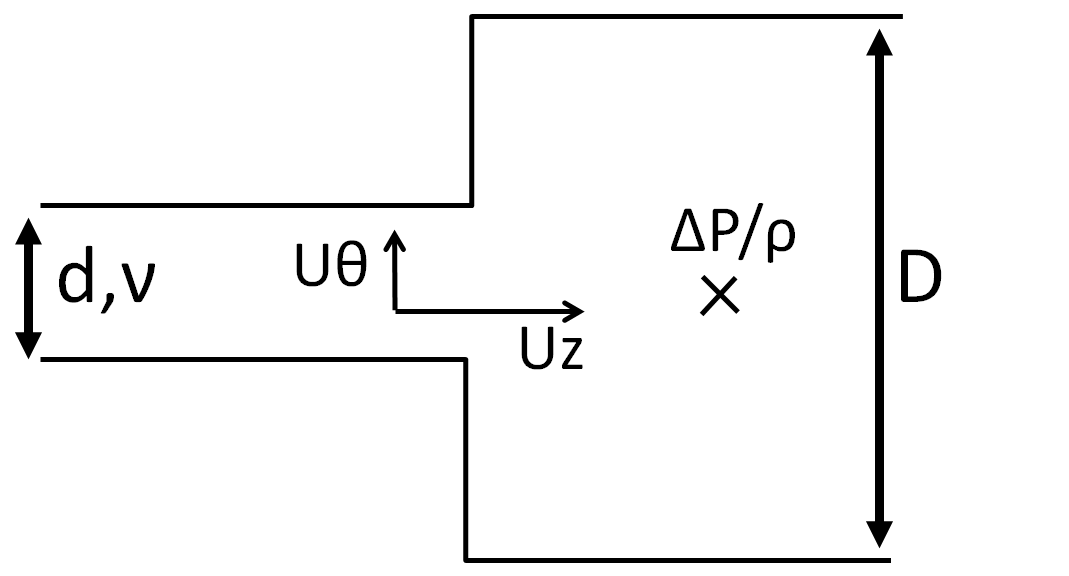
\includegraphics[width=0.6\textwidth]{fig/Schema_Vashy1.png}
  \caption{Basic case}
 \label{Vaschy1}
\end{figure}
Given a burner of internal diameter $d$, with a bulk velocity $u_{z}$,a tangential velocity $u_{\theta}$ ,  followed by a combustion chamber of internal diameter $D$, and a fluid with a kinematic viscosity $\nu$, we want to describe the behavior of the non-reactive flow inside the furnace. For instance, we can study the quantity $\frac{\Delta P}{\rho}$ at a given point inside the combustion chamber, we can otherwise choose $u_{r}$or any physical values, the adimensional numbers will be the same.

We need hypothesis for the velocities : let's assume a top-hat axial velocity, and a solid block body rotation, giving the shape :$u_{\theta}=\Omega r$. Let us use the Vaschy-Buckingham Theorem : we assume that the flow (through the quantity $\frac{\Delta P}{\rho}$ for example, or any else ) only depends on the previous data. 

Since we have 5 independent inputs ($d$,$\nu$,$u_{z}$,$\Omega$,$D$) with 2 units ($m$,$s$), there are $5-2=3$ adimensional numbers which fully describes the non-reactive flow. We can guess them, or find it back with linear analysis :
\begin{itemize}
\item $Re$ 
\item $S=\frac{\Omega d}{u_{z}}$
\item $C=\frac{d}{D}$
\end{itemize}

The adimensional number $\frac{\Omega d}{u_{z}}$ is written $S$ because we find, to within a constant, the well-known swirl-number :$S=\frac{\int_{0}^{d/2} u_{\theta} u_{z} r^2 dr}{d/2\int_{0}^{d/2}  u_{z}^2 r dr}$ 

Consequently, the flow is only a function of $S$, $Re$ and $C$ .

\paragraph{Influence of the density}

It has been a shortcut not to consider the density in the previous case. If we assume that the flows depends also on the density, let us enumerate the input parameters, we have now 6 of them : $d$,$\mu$,$\rho$,$u_{z}$,$\Omega$,$D$, but we also have added $kg$ as a unit. Hence, we have the same number of adimensional units : $6-3=3$. This is an important case where this powerful theorem demonstrates that there are simple cases where the kinematic viscosity is enough to describe the fluid.

\section{In the case of non uniform fields depending on cylindrical coordinates}

\begin{figure}[!h]
  \centering
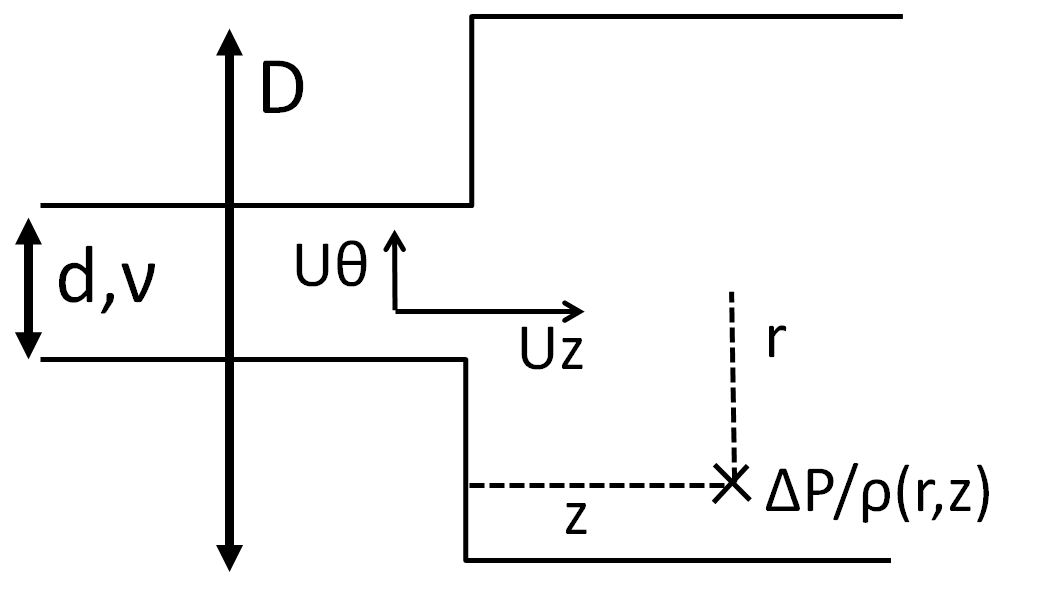
\includegraphics[width=0.6\textwidth]{fig/Schema_Vashy2.png}
  \caption{With cylindrical coordinates}
 \label{Vaschy2}
\end{figure}
In the previous case, the parameter $\frac{\Delta P}{\rho}$ has been considered as a macroscopic one, since not depending on $z$ and $r$ (let us assume the symmetry of rotation by neglecting $\theta$) . Let us now consider the case where we want to study a field depending on cylindrical coordinates : now $\frac{\Delta P}{\rho}(r,z)$. 

If we use the same approach, we easily see that there are 2 more unknown, with the same amounts of units, we have just added two adimensional coordinates to the problem, for instance $r/D$ and $z/D$. The input physical parameters driving the phenomena are the same. Hence, this is not absurd not to consider some coordinates, but we still have to know that the field will depend on adimensional coordinates.

Here, we have : $\frac{\Delta P}{\rho}(r,z)=f(\frac{r}{D},\frac{z}{D},Re,S,\frac{d}{D})$

From now on, let us not consider the dependency of the cylindrical coordinates.

\section{With a quarl angle}

Since Paul Jourdaine \cite{paul_jourdaine_nom_effect_2016} has now shown the huge dependency on the flow of the quarl angle, we can add it in our dimensional analysis.

\begin{figure}[!h]
  \centering
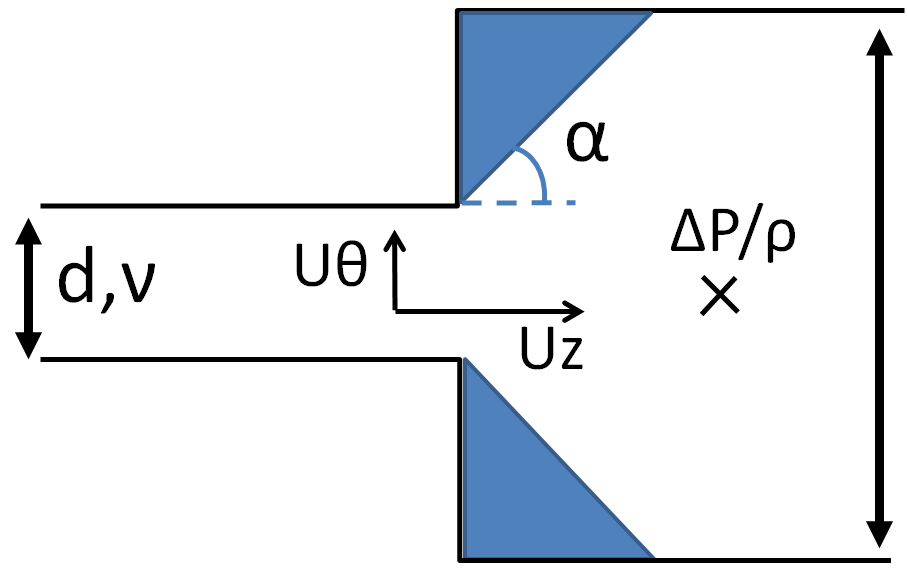
\includegraphics[width=0.6\textwidth]{fig/Schema_Vashy3.png}
  \caption{With quarl angle}
 \label{Vaschy3}
\end{figure}

The Vacshy-Buckingham analysis gives easily : that the quarl number is itself an adimen
sional number, we now have :
$\frac{\Delta P}{\rho}=f(\alpha,Re,S,\frac{d}{D})$

\section{Two coaxial swirled flows}

The new case deals with two flows, as presented in \ref{Vaschy4}. One common adimensional number we can find in the literature is the impulsion ratio : $J=\frac{\rho_{1} u_{1}^2}{\rho_{2} u_{2}^2}$ . In that case, one understands that the two densities will now influence the behavior of the flow. Thus, $\rho_{1}$ and $\rho_{2}$ must be counted on the inputs. We introduce here a new units, $kg$. 
\begin{figure}[!h]
  \centering
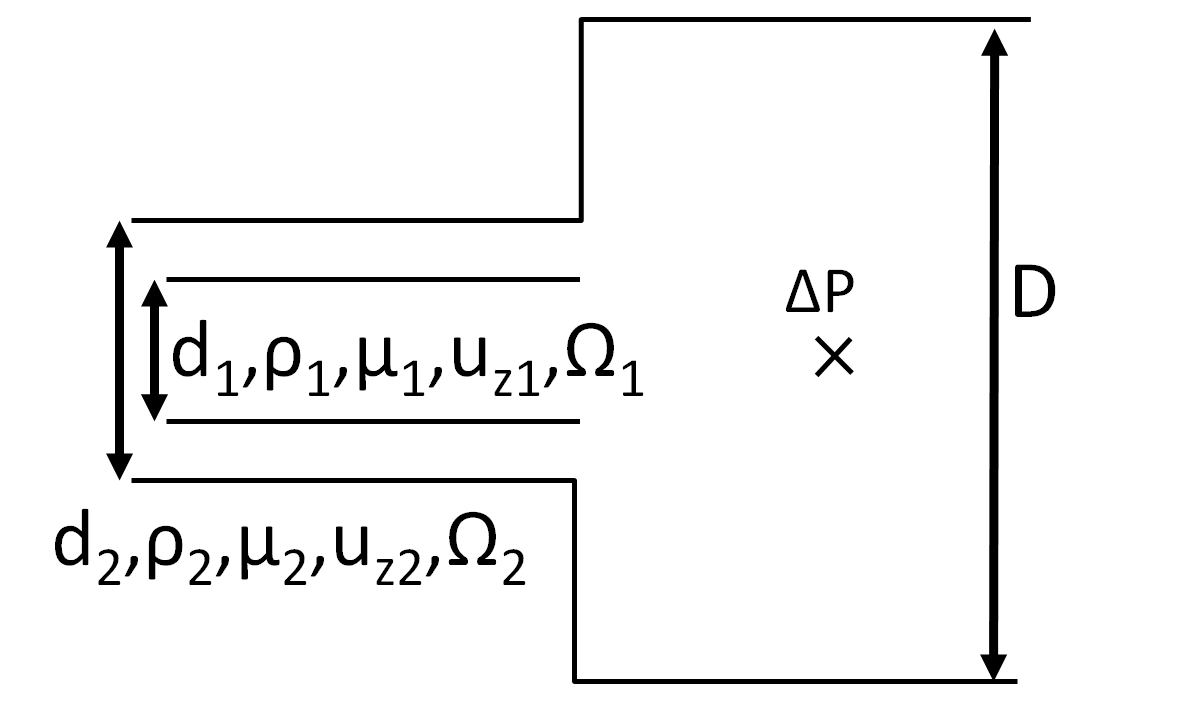
\includegraphics[width=0.6\textwidth]{fig/Schema_Vashy4.png}
  \caption{Two coaxial swirled flows}
 \label{Vaschy4}
\end{figure}
According to \ref{Vaschy4}, each flow at the inlet is fully described with the diameter $d$ (or equivalent diameter for the outer flow), the density $\rho$, the dynamic viscosity $\mu$ and the velocity flow (the axial velocity supposed as top-hat velocity $u_{z}$, and the tangential velocity supposed as solid block rotation, so that the vorticity $\Omega$ fully describes the tangential flow :  $u_{\theta}=\Omega r$). Hence, we have 5 input parameters for each flow, and the diameter $D$ of the combustion chamber. With 3 units ($m$,$kg$ and $s$), the Vaschy-Buckingham theorem gives that $11-3=8$ adimensional numbers fully describes the behavior of the flow :

Here are the chosen parameters : 

$Re_{1}$,$Re_{2}$,$S_{1}$,$S_{2}$,$\frac{d_{1}}{D}$,$\frac{d_{2}}{D}$,$J=\frac{\rho_{1} u_{z1}^2}{\rho_{z2} u_{2}^2}$,$\frac{\mu_{1}}{\mu_{2}}$. 

One can easily check that any new adimensional number is a combination of the previous ones : 

For instance, we could have chosen $\frac{u_{z1}}{u_{z2}}$ instead of $J$, but we have the relation : $J=\frac{Re_{1}}{Re_{2}} \cdot \frac{u_{z1}}{u_{z2}} \cdot \frac{\mu_{1}}{\mu_{2}}$ 

Hence, the non-reactive flow might be fully studied with a parametric study of these 8 adimensional numbers.

\section{Sizing of the strioscopy experiment}
\subsection{The approach}
As far as it is possible, we want the adimensional numbers to remain the same: $\frac{d_{1}}{D}$,$\frac{d_{2}}{D}$,$Re_{1}$,$Re_{2}$,$S_{1}$,$S_{2}$,$J$ and $\frac{\rho_{1}}{\rho_{2}}$. We also want to use the same velocities as the ones in HPPOX. 

According to our hypothesis to consider the geometrical swirl number, we see that the use of the same ATR-30norm burner automatically gives that $\frac{d_{1}}{D}$,$\frac{d_{2}}{D}$,$S_{1}$ and $S_{2}$ remain the same. (Let us neglect in a first approach the fact that we will not use any combustion chamber in the strioscopy diagnostic, so that the diameter $D$ is not defined anymore). 

Hence, we have to choose our inlet gases in order to keep as constant as possible the quantities : $Re_{1}$,$Re_{2}$,$J$ and $\frac{\rho_{1}}{\rho_{2}}$. Unfortunately, other conditions make the conservation of these adimensional quantities all the more difficult :
\begin{itemize}
\item To increase the efficiency of the strioscopy, one needs a high density gradient, implying that we need   $\frac{\rho_{2}}{\rho_{1}}$ far from the unity. "far" still needing to be defined. By heating air at $100^\circ C$, Y. Joumani (ref) had a density ratio of 1.27, which apparently was not enough. Fortunately, since we want to approach $\frac{\rho_{1}}{\rho_{2}}$ from the experiment on Calhory, the value reaches $\frac{\rho_{O_{2}}}{\rho_{CH_{4}}}_{Freiberg}=3$ , which may be enough to have useful density gradients.
\item Dealing with the experiment, heating the gases or diluting them make the experiment more difficult to implement. Particularly, though it would be an efficient solution, using natural gas without combustion chamber nor furnace seems unsafe.
\end{itemize}

\section{Sizing of the Calhory experiment}

The main difference is that the kinetic aspect also need to be considered here, since there the combustion phenomenon is now effective. The Vaschy-Buckingham analysis with a non-reactive flow  gave adimensional numbers to be conserved. It seems difficult to use the same approach to make kinetic adimensional numbers appear :

\begin{itemize}
\item There are many more unknown to the problems and free parameters (every fraction of each specie in each flow, and we are just adding the temperature as dimension
\item In order to use the Vaschy-Buckingham theorem, the main idea is to assume the parameters from the beginning that will be involved in a certain metric we want to observe. Here, non only the determination of the  involved parameters are exactly the scientific problem the internship wants to tackle, but also it is very hard to define a single metric to observe the flame (should it be the flame length, the width, the maximum temperature...?)
\end{itemize}
Consequently, the bibliography has been widely investigated in order to define the main parameters. Let us not forget that the idea is not the predict the flame length, but to make sure that the identified parameters are conserved between Freiberg and the Calhory experiment.

The simplest investigation is the laminar case : in (\# ref Veynante), the length of a diffusion flame in the laminar case is $L_{f}=\frac{e_{0}Re}{2\pi}\cdot \frac{1}{Z_{st}^2}$  with $e_{0}$ a geometrical length. We know in that a ratio of 40 will change the pressure, so the Reynolds $Re$, but Veynantes also says that the flame length in turbulence flow does not depend on the Reynolds. Hence, the important parameter here is $Z_{st}$, and it is the one we want to keep constant. According to (\#ref Peters), a clear definition of $Z_{st}$ can be : $Z_{st}=(1+\frac{\nu Y_{F,1}}{Y_{O_{2},2}})^{-1}$ where $\nu$ is the mass stoechiometric ratio (4 for $CH_{4}-O_{2}$ flame),    $Y_{F,1}$ the mass ratio of fuel in the fuel injection ($Y_{F,1}=1$ if it is pure $CH_{4}$) and $Y_{O_{2},2}$ the mass ratio of oxygen in the oxydant injection ($Y_{O_{2},2}=0.23$ if it is pure air).

Consequently, we choose the $Z_{st}$ to be constant. In Freiberg, $Z_{st}=0.31$.


\newpage

\section{Investigation on Optisos analysis }

\subsection{Context of the investigation}

Given the lack of experimental data one is faced with in terms of ATR combustion. The experiments on Freiberg HP-POX burner are almost our only contact with industrial real results of combustion process in ATR burner. Furthermore, a detailed campaign has been made with parametric study of different inputs, such as the S/C ratio, the load variation or the Oxygen/NG velocity ratio. The chosen metric to investigate the flame topology here will be the flame length 

The conclusion of the report are that :
\begin{enumerate}
\item Changing the pressure of the ATR burner from 30 to 50 bars leads to small variation of the flame length
\item The S/C ratio is the parameter that the biggest impact on the flame topology : With a S/C ratio increasing from 1 to 1.4, the flame length decreases from 124mm to 84mm
\item The burner load also drives the flame length : increasing burner load shortens the flame
\item High temperatures of the reactor leads to longer flame
\end{enumerate}

In order to emphasize the conclusion of the reports, here are the corresponding plot from Optisos report :

\begin{figure}[h!]
  \centering
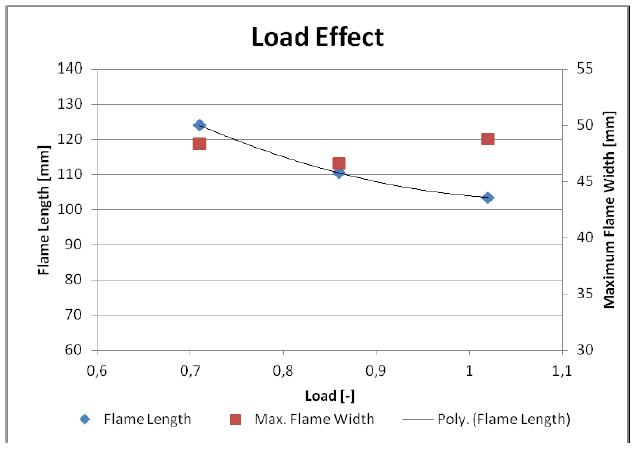
\includegraphics[width=0.45\textwidth]{fig/Optisos_Load_effect.PNG}
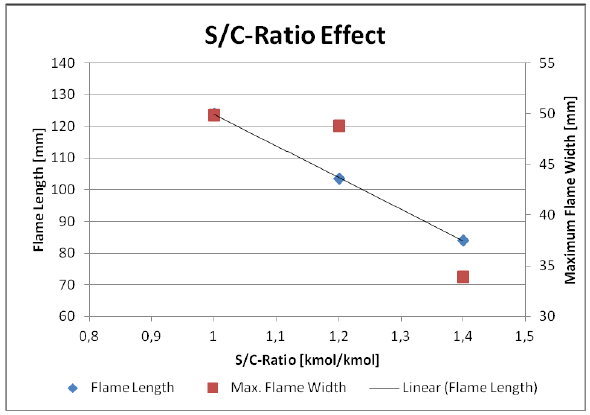
\includegraphics[width=0.45\textwidth]{fig/Optisos_S_C_effect.PNG}
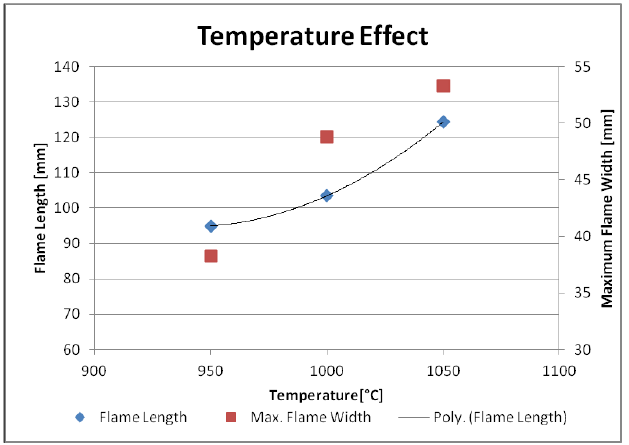
\includegraphics[width=0.45\textwidth]{fig/Optisos_temperature_effect.PNG}
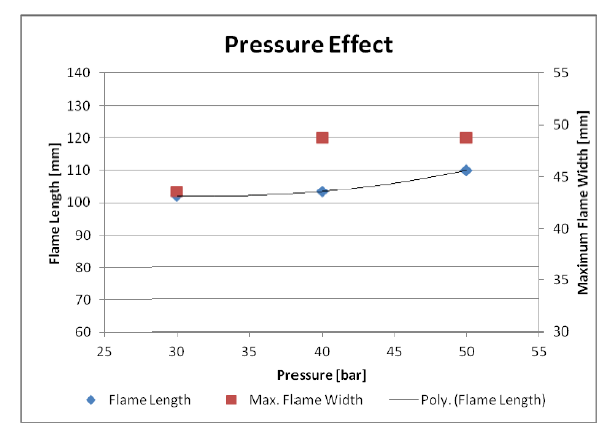
\includegraphics[width=0.45\textwidth]{fig/Optisos_Pressure_effect.PNG}
  \caption{Conclusion of Optisos report on flame topology}
 \label{optisos_plot}
\end{figure}

Dealing with my internship, if the flame length depended on so many parameters, it mean that I would have to study them all, and to keep them constant in Calhory burner with scales-up rule. This task seems impossible to achieve. Besides, a analysis of  the literature gives another interpretation. 

In a the laminar case : in (\# ref Veynante), the length of a diffusion flame in the laminar case is $L_{f}=\frac{e_{0}Re}{2\pi}\cdot \frac{1}{Z_{st}^2}$  with $e_{0}$ a geometrical length. With  $Z_{st}=(1+\frac{\nu Y_{F,1}}{Y_{O_{2},2}})^{-1}$ where $\nu$ is the mass stoechiometric ratio (4 for $CH_{4}-O_{2}$ flame),    $Y_{F,1}$ the mass ratio of fuel in the fuel injection ($Y_{F,1}=1$ if it is pure $CH_{4}$) and $Y_{O_{2},2}$ the mass ratio of oxygen in the oxidant injection ($Y_{O_{2},2}=0.23$ if it is pure air). 

In an analysis from (\# ref Peters), in a case with static oxidant and a non swirled fluel flow, Peters demonstrates the flame length :$\frac{L+x_{0}}{d}=\frac{2.19 (1+2Sc)}{Z_{st}}\frac{\rho_{0}}{\rho_{st}C}$, while another (\# ref) gets experimentally the length  $\frac{L+x_{0}}{d}=\frac{5.3}{Z_{st}}(\frac{\rho}{\rho_{st}})^{-1/2}$.

The purpose of these formulas is obviously not to use them for a much more complicated case (swirled coaxial flow), but to consider that all the parametric parameters studied in Optisos report can be gathered with adimensional number. If these formula were correct, the flame length should depend on the stoichiometric mixture fraction $Z_{st}$, since $Z_{st}$ keeps all the information of S/C dilution, burner load or pressure variation of density.

Hence, the data from Optisos has been re-used to compute in each test the corresponding $Z_{st}$, and it has be found that, in the area of the tests that have been conducted, the flame length of ATR burner measured in Optisos diagnostic directly depends on the stoichiometric mixture fraction $Z_st$ as an affine function :

The points in red are the cases where the temperature of the reactor has been changed, which does not implicate the $Z_{st}$, and adresses heat transfer and kinetic.

\begin{figure}[h!]
  \centering
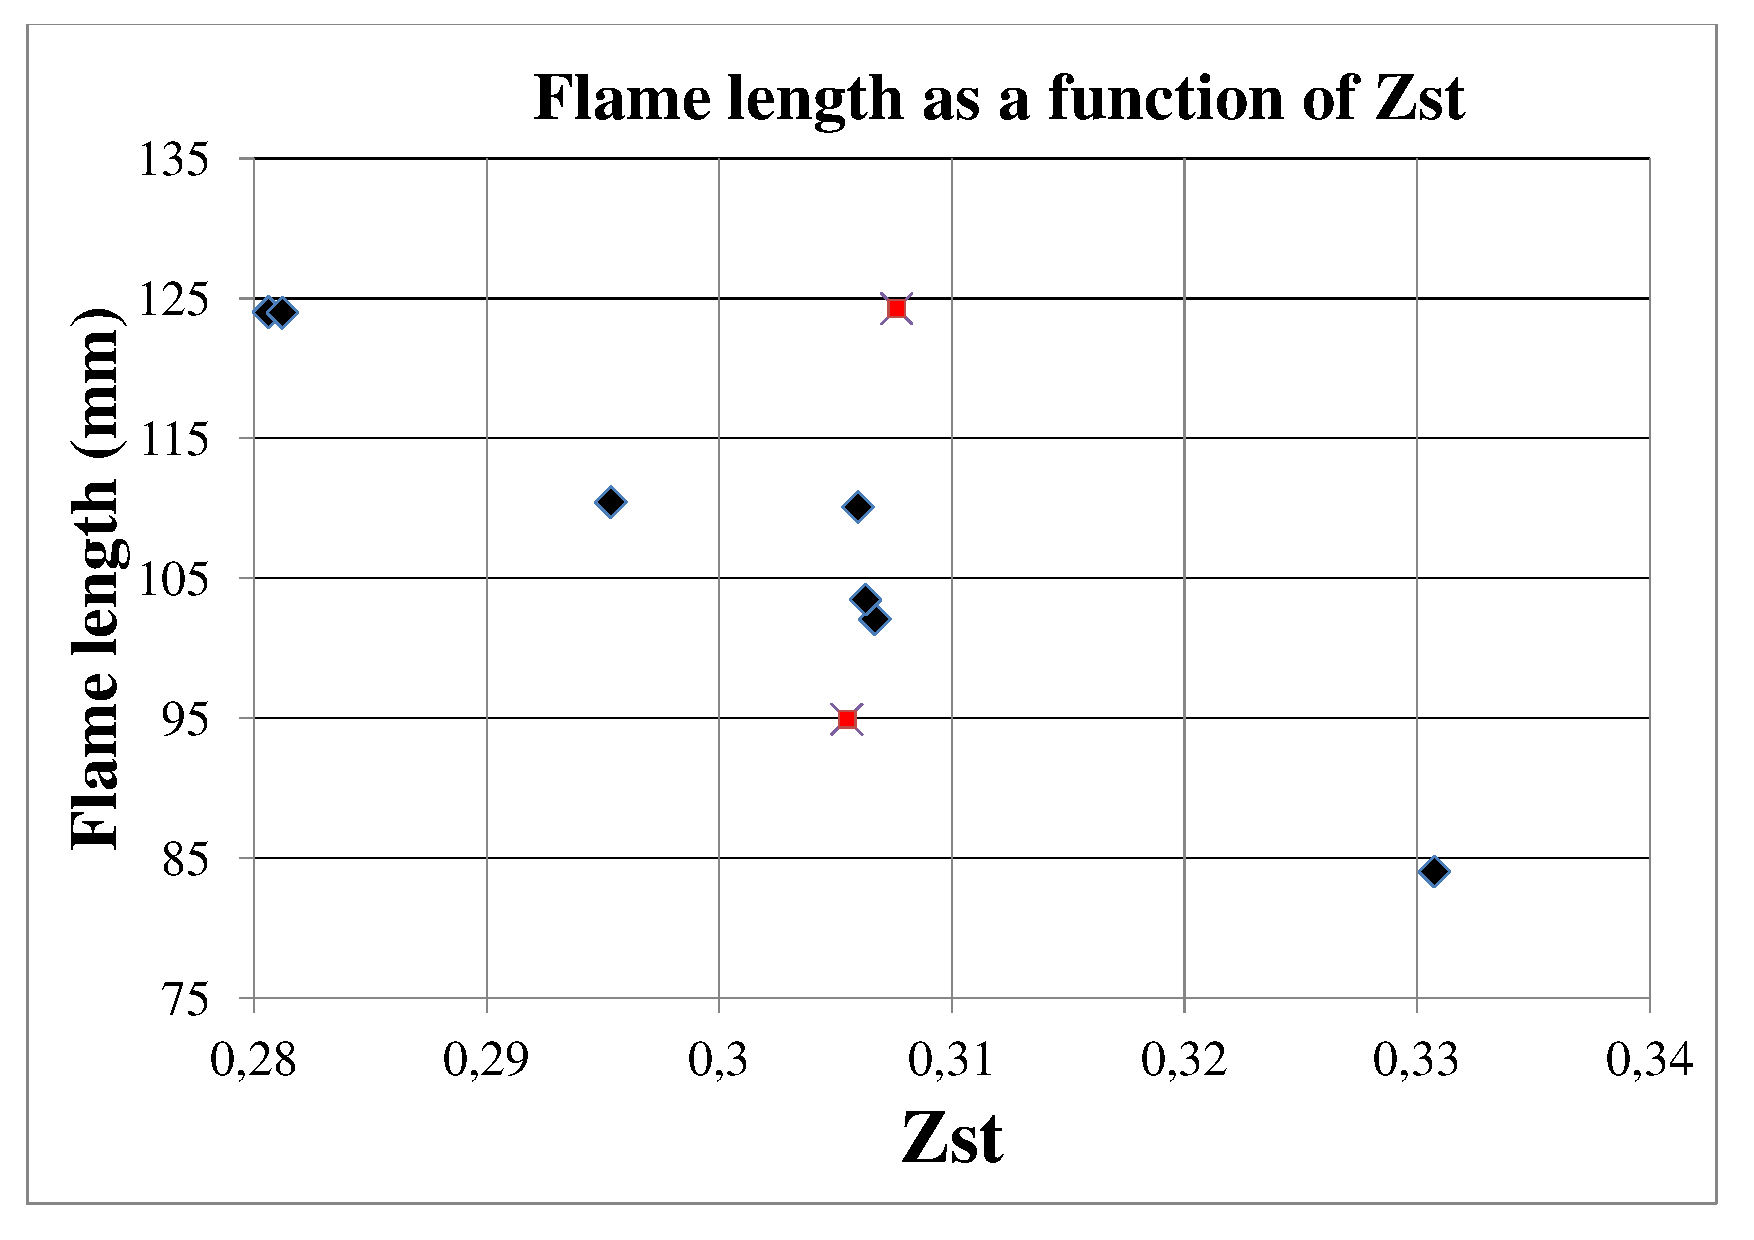
\includegraphics[width=0.8\textwidth]{fig/Flame_length_Zst.pdf}
 \label{Flame length as a function of Zst}
\end{figure}

It would be interested to get more points, or to extend the investigation segment, to define a characteristic law such as $Length=A_{0}-A_{1}\cdot Z_{st}$. One can easily verify that the trend is logical according to what have been observed previously, 
\renewcommand\evenpagerightmark{{\scshape\small Filière Work for Centrale}}
\chapter[Partie filière]%
{Partie filière}
\label{Partie filière}

\section{Partie filière}

\section{Besoins industriels d'Air Liquide}

Air Liquide utilise la combustion pour produire des gaz industriels comme l'hydrogène ou le monoxyde de carbone. Ces gaz sont les matières premières indispensables à bon nombres d'industries chimiques, notamment la pétrochimie. L'activité première d'Air Liquide étant de vendre des contrats de l'oxygène qu'elle produit, l'activité combustion d'Air Liquide ne se fait pas à l'air mais avec de l'oxygène (on a retiré l'azote de l'air) : c'est le principe d'oxycombustion. Cette technologie permet également d'atteindre des températures plus élevées qu'à l'air, d'améliorer le rendement du combustible, ainsi que de limiter significativement les émissions polluantes.
    
Les fours produisant ce mélange monoxyde de carbone/hydrogène sont appelés fours AutoThermal Reforming (ATR). Ils ont été dimensionnés par la société Lurgi, rachetée par Air Liquide en 2007. Aujourd'hui, les règles de dimensionnement des fours ATR sont mal maîtrisées. L'ingénierie n'est pas encore prédictive et la conception manque d'outils pour dimensionner les brûleurs. Air Liquide veut donc davantage maîtriser les process dans le but de :
\begin{itemize}
\item Augmenter la production en sortie de gaz
\item Maîtriser davantage les rejets
\item Diminuer le coût de dimensionnement des fours (CAPEX) ou augmenter l'efficacité de la conversion du fuel en gaz de synthèse (OPEX)
\item Obtenir des gaz de meilleurs qualités
\end{itemize}

Dans ce but, un pilote a été construit en 2004 à Freiberg. De nombreux tests ont été conduits sur ce brûleur et ces données sont le point de départ du stage.


A travers mon stage stage, Air Liquide désire :
\begin{itemize}
\item Obtenir des règles de dimensionnement pour les brûleur ATR : lois d'échelles par des nombres adimensionnés adaptés, justifier les choix technologiques de Lurgi
\item Comprendre le comportement des flammes et les mécanismes responsables
\item Donner de la visibilité à la recherche numérique, qui manque aujourd'hui cruellement de données expérimentales pour justifier les modèles
\end{itemize}



\subsection{L'ATR au sein de la R\&D aux loges}

 Peu de travaux ont été conduits sur les fours ATR, et la majorité concerne l'équipe de mathématiques appliquées. Les volumes de fours ATR vendus dans le monde sont aujourd'hui faibles mais sont toujours des investissements conséquents. Air Liquide s'intéresse de nouveaux aux ATR depuis le rachat de Lurgi mais l'appropriation et la remise en questions de la conception des ATR nécessite du temps.

\section{Déroulé et plans du stage}


En terme de gestion de projet, mon stage s'insère dans un programme de recherche plus général : la chaire Oxytec a été créée entre Air Liquide et le laboratoire EM2C de Centrale pour investiguer le comportement des flammes d'Air Liquide, qui sont très atypiques (haute pression, combustion de l'oxygène, éventuelles dilutions...). La chaire a financé six thèses dont l'objectif final est de fournir des outils numériques et un banc d'essai de haute précision permettant de reproduire et observer les flammes industrielles (ce qui requiert des moyens très conséquents et n'a jamais pu être réalisé auparavant). Au sein de ce programme, mon stage amorce la réflexion sur les véritables brûleurs utilisés dans les procédés Air Liquide. Il est en très forte relation avec la dernière thèse que le projet Oxytec a prévue, thèse pour laquelle je suis aujourd'hui le candidat d'Air Liquide et du EM2C.

Il est nécessaire de comprendre pourquoi l'étude des flammes n'est pas encore maîtrisée aujourd'hui :
\begin{itemize}
\item D'un point de vue numérique, résoudre les équations d'une flamme requiert des moyens de calculs inaccessibles même aux plus grands super-calculateurs mondiaux.
\item D'un point de vue expérimental, étudier une flamme de taille industrielle (pression et puissance très élevées : 40 bar, 5MW) est à la fois prohibitif dans le prix et inaccessible expérimentalement puisque il est impossible de placer des capteurs dans des flammes industrielles
\end{itemize}

La stratégie est donc de recourir aux lois d'échelles : par un dimensionnement judicieux, on veut montrer qu'on peut se rapporter à des flammes de laboratoires (néanmoins très importantes), mais qu'on peut analyser. C'est le premier objectif de mon stage : retrouver la flamme du pilote industriel de Freiberg par l'analyse des phénomènes.

Si cet objectif est rempli, alors on aura la légitimité pour étudier l'influence de paramètres qui n'ont vraisemblablement pas été étudiés lors de la conception des brûleurs.Par exemple, en changeant simplement certains débits judicieusement ou le design du brûleur, on espère pouvoir piloter les caractéristiques de la flamme.

\subsection{Ce qui a été réalisé}

J'ai été confronté dès le début à toutes les contraintes d'ordre industriel sur lesquels j'avais assez peu d'emprise : les délais pour lancer des campagnes d'essais sont très longues, il faut attendre la disponibilité des techniciens et des fours. C'est pourquoi, avec mes connaissances issues du master, j'ai proposé au centre un nouveau moyen de diagnostic des écoulements, qui est beaucoup moins contraignant en terme de sécurité et de planning. Cela m'a permis de gagner du temps et de l'indépendance sur mes campagnes d'essais, que j'ai pu démarrer assez vite après le début de mon stage. Ce diagnostic repose sur l'étude des écoulements à froid par interférométrie et son apport au centre constituera un réel atout si mes résultats s'avèrent concluants (ce sur quoi je suis très optimiste).

Ma contribution scientifique a beaucoup porté au début sur l'établissement de règles de dimensionnement pour retrouver les caractéristiques de flammes industrielles à partir de flammes de laboratoires. Pour cela, la bibliographie a été largement consultée et analysée. Ces règles de dimensionnement sont finies, et seront mises à l'épreuve lorsque les premiers tests seront menés. Mon traitement de campagnes d'essais précédemment menées sur le brûleur industriel de Freiberg donne des résultats très encourageants pour mes règles de dimensionnement.

Un brûleur prototype a également été dimensionné et conçu à partir de zéro pour étudier l'injection de l'oxygène. Il est en cours d'impression 3D et sera utilisé en août. 



\subsection{Réflexion sur la gestion de projets au sein du stage}

La réflexion expérimentale que je mène sur les brûleurs ATR industriels d'Air Liquide part presque de zéro, et les durées des projets R\&D sont souvent bien supérieures à 6 mois. De plus, mon stage étant à dominante expérimentale, l'utilisation de fours de grosses puissances dépend énormément des fours disponibles au centre, de la disponibilité des techniciens, de l'approvisionnement en gaz des laboratoires, de la fabrication à temps des pièces nécessaires, des contraintes de sécurité très spécifiques à l'entreprise. L'aspect organisationnel est donc critique et un soin très important est porté à l'anticipation des risques, à la discussion avec toutes les parties prenantes pour l'anticipation.

Ma démarche est de constamment prendre des marges d'emploi du temps, privilégier les choix technologiques ou stratégiques où je suis le plus indépendant des contraintes extérieures (sécurité, disponibilité du matériel et des techniciens). C'est avec ce souci d'optimisation du temps que j'ai tenu à mesurer mes écoulements à froid de manière indépendante, ce qui s'est avéré judicieux dans la mesure ou la disponibilité des fours a effectivement pris du retard.

\subsection{Risques et opportunités}

Malgré mes efforts, les principaux risques sont liés à la disponibilité des ressources (humaines et matérielles). Faiblement probables, une indisponibilité totale des plusieurs fours qui ont été envisagés m'empêcheraient d'obtenir les résultats de combustion, ce qui serait très négatif pour le déroulé du stage. Des moyens de mitigations sont continuellement recherchés.

Un risque important porte également sur l'invalidité d' une hypothèse scientifique que la direction scientifique et moi-même avons prise. Si le temps de la chimie n'est pas court devant la turbulence, il sera très difficile de retrouver les flammes industrielles avec mes lois d'échelles.

Deux opportunités se présentent. La première est l'apport d'un nouveau diagnostic de mesure au centre Air Liquide : si l'interférométrie des écoulements à froid est concluante, le laboratoire peut envisager des applications à mon dispositif expérimental.

La deuxième concerne les perspectives de l'utilisation des lois d'échelles : si je peux retrouver une flamme industrielle sur un four de laboratoire, les phénomènes pourront être étudiés avec beaucoup plus de légitimité.

\subsection{Planning à jour}

En vert le travail accompli, en rouge les retards dues aux contraintes industrielles, et en orange la prévision. A noter que chaque chemin est critique dans sa catégorie, les campagnes d'essais ne pouvant être fait si le matériel n'arrive pas à temps. Le moi d'octobre n'a pas été rempli : dans le cas le plus pessimiste, il servira à rattraper le retard du à la disponibilité des ressources, dans le cas le plus optimiste, de nouveaux tests plus approfondis seront menés.

\begin{figure}[!h]
  \centering
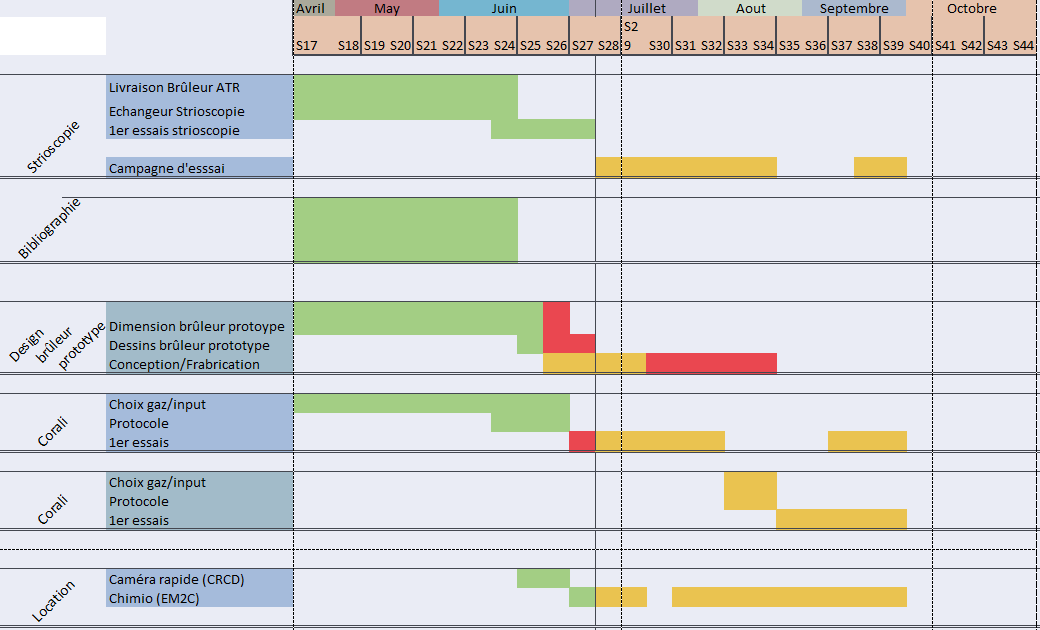
\includegraphics[width=0.9\textwidth]{fig/Gantt_Intermediaire.PNG}
  \caption{Diagramme de Gantt intermédiaire}
 \label{Gantt Int}
\end{figure}
\begin{figure}[!h]
  \centering
\includegraphics[width=0.40\textwidth]
{fig/com/timetable.png}

  \caption{Typical ISO sensitivity}
 \label{fig_Iso_sensitivity_1D}
\end{figure}


Le stage c'est aussi :
\begin{itemize}
\item 60 heures devant le four
\item 2 fois la consommation électrique annuelle d'un couple (sans chauffage)
\item x heures des calcul LES
\item 5 techniciens trop aidants
\item 4 diagnostics optiques différents utilisés
\end{itemize}
\renewcommand\evenpagerightmark{{\scshape\small Diagnostic}}
\chapter[DiagnosticMeasurement]%
{DiagnosticMeasurement}
\label{diagnostic_chapt}

\section{Strioscopy}

\subsection{Opportunities}

What we would like to measure :

\begin{itemize}
\item velocity field
\item density field
\item turbulence field
\item mixture field
\item recirculation zone
\end{itemize}

What we are sure we can measure if the experiments works perfectly  :

\begin{itemize}
\item qualitative representation of the mixture
\item qualitative idea of the turbulence 
\item recirculation zone
\end{itemize}



\subsection{According to the user guide}

Possible to compute quantitatively the density, the temperature (assuming that we know the pressure), even some velocity values... It is very well described, the calculations are very long and not automatized in a script (feasibility?)

\section{Procedure}

\subsection{What is needed}

\begin{itemize}
\item The strioscopy
\item a dilution facility 
\item A thermocouple
\item A calibrated movable pedestal
\item A CCD camera (when the whole diagnostic is proven to work)
\item The preheater
\item An area of $4m * 2m$
\item Gaz supply (air?) at the right velocity
\item a table, a meter
\end{itemize}
\section{Dimensional analysis}
\subsection{The approach}
As far as it is possible, we want the adimensional numbers to remain the same: $\frac{d_{1}}{D}$,$\frac{d_{2}}{D}$,$Re_{1}$,$Re_{2}$,$S_{1}$,$S_{2}$,$J$ and $\frac{\rho_{1}}{\rho_{2}}$. We also want to use the same velocities as the ones in HPPOX. 

According to our hypothesis to consider the geometrical swirl number, we see that the use of the same ATR-30norm burner automatically gives that $\frac{d_{1}}{D}$,$\frac{d_{2}}{D}$,$S_{1}$ and $S_{2}$ remain the same. (Let us neglect in a first approach the fact that we will not use any combustion chamber in the strioscopy diagnostic, so that the diameter $D$ is not defined anymore). 

Hence, we have to choose our inlet gases in order to keep as constant as possible the quantities : $Re_{1}$,$Re_{2}$,$J$ and $\frac{\rho_{1}}{\rho_{2}}$. Unfortunately, other conditions make the conservation of these adimensional quantities all the more difficult :
\begin{itemize}
\item To increase the efficiency of the strioscopy, one needs a high density gradient, implying that we need   $\frac{\rho_{2}}{\rho_{1}}$ far from the unity. "far" still needing to be defined. By heating air at $100^\circ C$, Y. Joumani (ref) had a density ratio of 1.27, which apparently was not enough. Fortunately, since we want to approach $\frac{\rho_{1}}{\rho_{2}}$ from the experiment on Calhory, the value reaches $\frac{\rho_{O_{2}}}{\rho_{CH_{4}}}_{Freiberg}=3$ , which may be enough to have useful density gradients.
\item Dealing with the experiment, heating the gases or diluting them make the experiment more difficult to implement. Particularly, though it would be an efficient solution, using natural gas without combustion chamber nor furnace seems unsafe.
\end{itemize}

\subsection{The dimension calculation }
An Excel tool has been created to compare the HPPOX values and the strioscopy diagnostic. As a preliminary conclusion, the theoretical best option would be to use natural gas and air at ambient temperature. Since the unburnt natural gas may be forbidden, another option would be to use air/air and burn the inner air at $200 ^\circ C$ , the adimensional numbers would be quite accurate, except the inner Reynolds number$Re_{1}$. One can refer to the Excel sheet for more details. 

With Python, a parametric study may be conducted to explore all the possibilities and analyze if there is not a better option to match the adimensional numbers.

In order to mitigate the conclusion, since we do not expect, for now, a very accurate comparison, nor a very precise quantitative diagnostic, we may not need to respect these adimensional numbers with such an accuracy. 

\subsection{Operational concerns}

\begin{figure}[!h]
  \centering
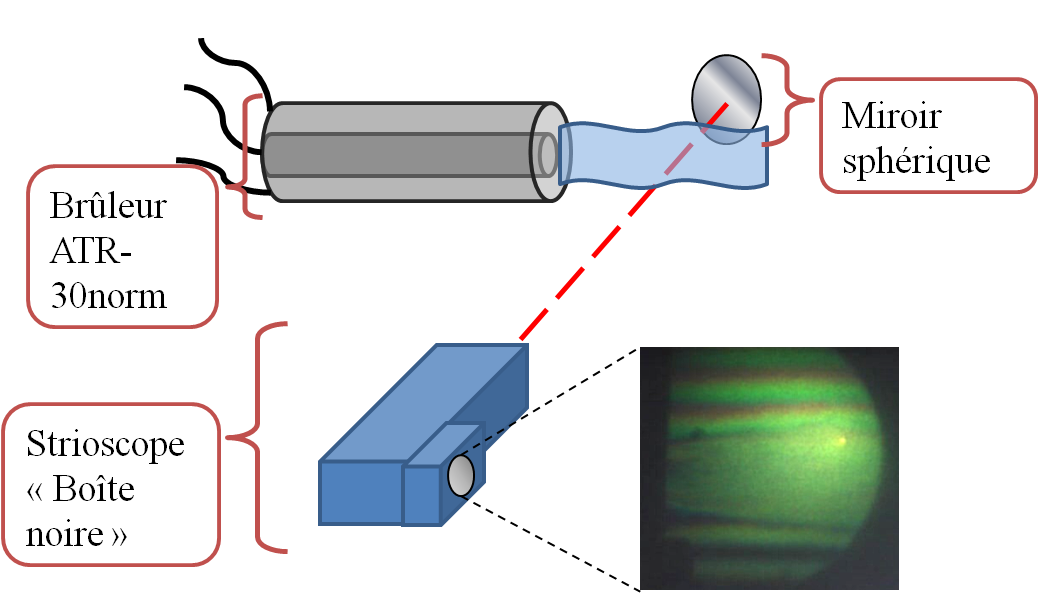
\includegraphics[width=0.6\textwidth]{fig/Schema_strio.png}
  \caption{The strioscopy experiment}
 \label{schema_strio}
\end{figure}
\subsubsection{The diagnostic of strioscopy }

There many kinds of strioscopy, the global aim is to measure the difference of optical path between two coherent beams. A difference of optical path induce a difference of density according to Gladstone-Dale law : $n-1=\kappa  \rho$. 

The strioscopy available at CRCD is interferential strioscopy, whose principle is described here :
\begin{figure}[!h]
  \centering
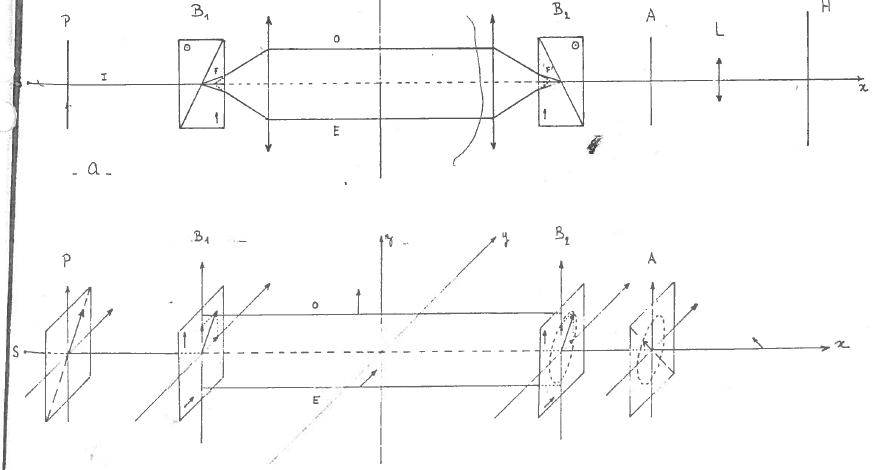
\includegraphics[width=0.8\textwidth]{fig/Principe_Strio.PNG}
  \caption{The strioscopy diagnostic}
 \label{principe_strio}
\end{figure}
A mercury source light (S) polarized by a polarizer (P) is divided into two coherent beams with a 1st biprism (B1). If the optical path between the two beams are equal, the 2nd biprism (B2) will gather the two beams, so that the polarization plan will be the same as before. A second polarizer works as an analyzer (A) : it  has a polarization plan perpendicular to the 1st polariszer, so that if the beam is not modified, no beam will be transmitted through the analyzer.

In case of a difference of optical path in the volume we want to measure, the polarization plan of the beam leaving the second biprism (B2) will not be the same, and its projection on the perpendicular polarization plan of the analyzer (A) will not be equal to zero anymore.

A fringe set up can be obtained by translating the second biprism along x-axis : without any perturbation of the measurement volume, the difference of optical path is then going to depend on the coordinate of the beam, so that parallel interferential fringes will appear in the absence of  perturbation of the measurement volume. The fringe set-up is responsible for the observation on figure \ref{image_strio} : when there is no pertubation, the fringes are strictly parallel, we can here observe a boundary layer at the proximity of the solid body thanks to the disposal.

\begin{figure}[!h]
  \centering
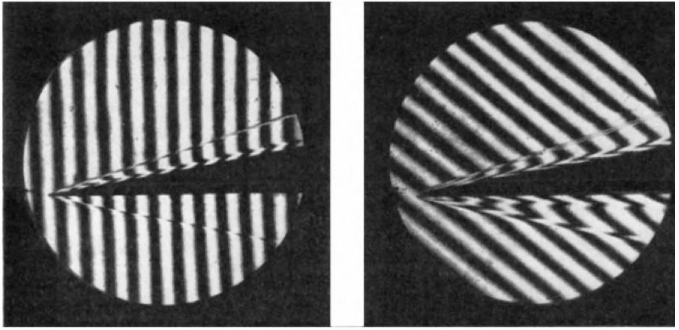
\includegraphics[width=0.8\textwidth]{fig/Strioscopie.PNG}
  \caption{The strioscopy diagnostic}
 \label{image_strio}
\end{figure}


\subsubsection{Procedure}

\begin{enumerate}
\item On a table, install the strioscope device
\item install the spherical mirror 3 meters ahead the lens of the strioscope
\item To calibrate the device, you can : \begin{itemize}
\item control the translation of the optical device (particularly, two configurations can be reached (by moving the strioscope along the optical axe): flat-colour or with fringe, in the case of fringes, one can change the position of the fringes by moving the biprism laterally)
\item choose the angle of the biprism ($1^\circ$,$2^\circ $ or $3^\circ$)
\item control the movement of the refringent bi-prism
\item In order to make the focus : control the drum with 8 positions for lenses, and then adjust it manually with the secondary fine controlling button (at the end of that point, the focus is supposed to be done on the examined object)
\item Change the device on which the final image is reflected (it can be a dulled glass, or a photographic plate, or a camera fixed to a support, or a screen)
\end{itemize}
\item One can check the set up with a small flame from a lighter
\end{enumerate}
\subsubsection{To take into account}
\paragraph{Protect the flow from the wind} It is absolutely necessary not to be under the influence of the wind. The best option is to make it indoor.

\paragraph{Taking care with the outlet temperature} Y. Joumani had troubles with keeping the outlet temperature because of the cooling inside the pipe. We have to measure it at the outlet (with thermocouple, for every used mass flow!) but also to insulate the pipes, or preheat a lot the initial gaz.

\paragraph{To test if the burner is really axisymetrical} Turn the burner and compare the results

\subsubsection{To include in the planning}
\begin{itemize}
\item CCD camera
\item Preheater
\end{itemize}
\section{The sizing of the reheater for the strioscopy}

  This is a compromise between the need for the experiment and the difficulty to craft the facility. This is a problem of heat transfer : with a given mass flow $\dot{m}=20.5 kg/h$, we want to heat air from ambient temperature to $T_{outlet}=605^\circ C$ with a hoven of maximal temperature $T_{hoven}=850^\circ C$. A simple OD model gives the energy balance :
  
  $\dot{m} c_{p} (T_{outlet} -T_{inlet})=(T_{hoven}-T_{mixture}) h S_{wet}$
  
  We use the correlation heat transfer : 
  
  $h=0.023 Re^{4/5} Pr^{0.3}$,  we introduce the length :$x_{0}=\frac{c_{p} \dot{m}^{1/5}D^{4/5}}{\lambda Pr^{0.3} 0.023 (4/(\mu \pi)^{4/5}\pi}$ 
 
and we find with a 0D model the necessary length $L$ to reach the outlet temperature : $L=x_{0} \frac{T_{outlet} -T_{inlet}}{T_{hoven}-T_{mixture}}$ 

and with a 1D model : $L=-x_{0} ln(1-\frac{T_{outlet} -T_{inlet}}{T_{hoven}-T_{inlet}})$  

The figure \ref{heater_sizing} shows that the two models are quite close at 1st order, we have to choose a technical solution with a reliable velocity (less than 30). Margins has been taken in this scenario, knowing that the pipe will not be at the exact temperature of the hoven, and that we want to over heat the flow at the outlet to compensate the thermal loss to reach the burner.

\begin{figure}[!h]
  \centering
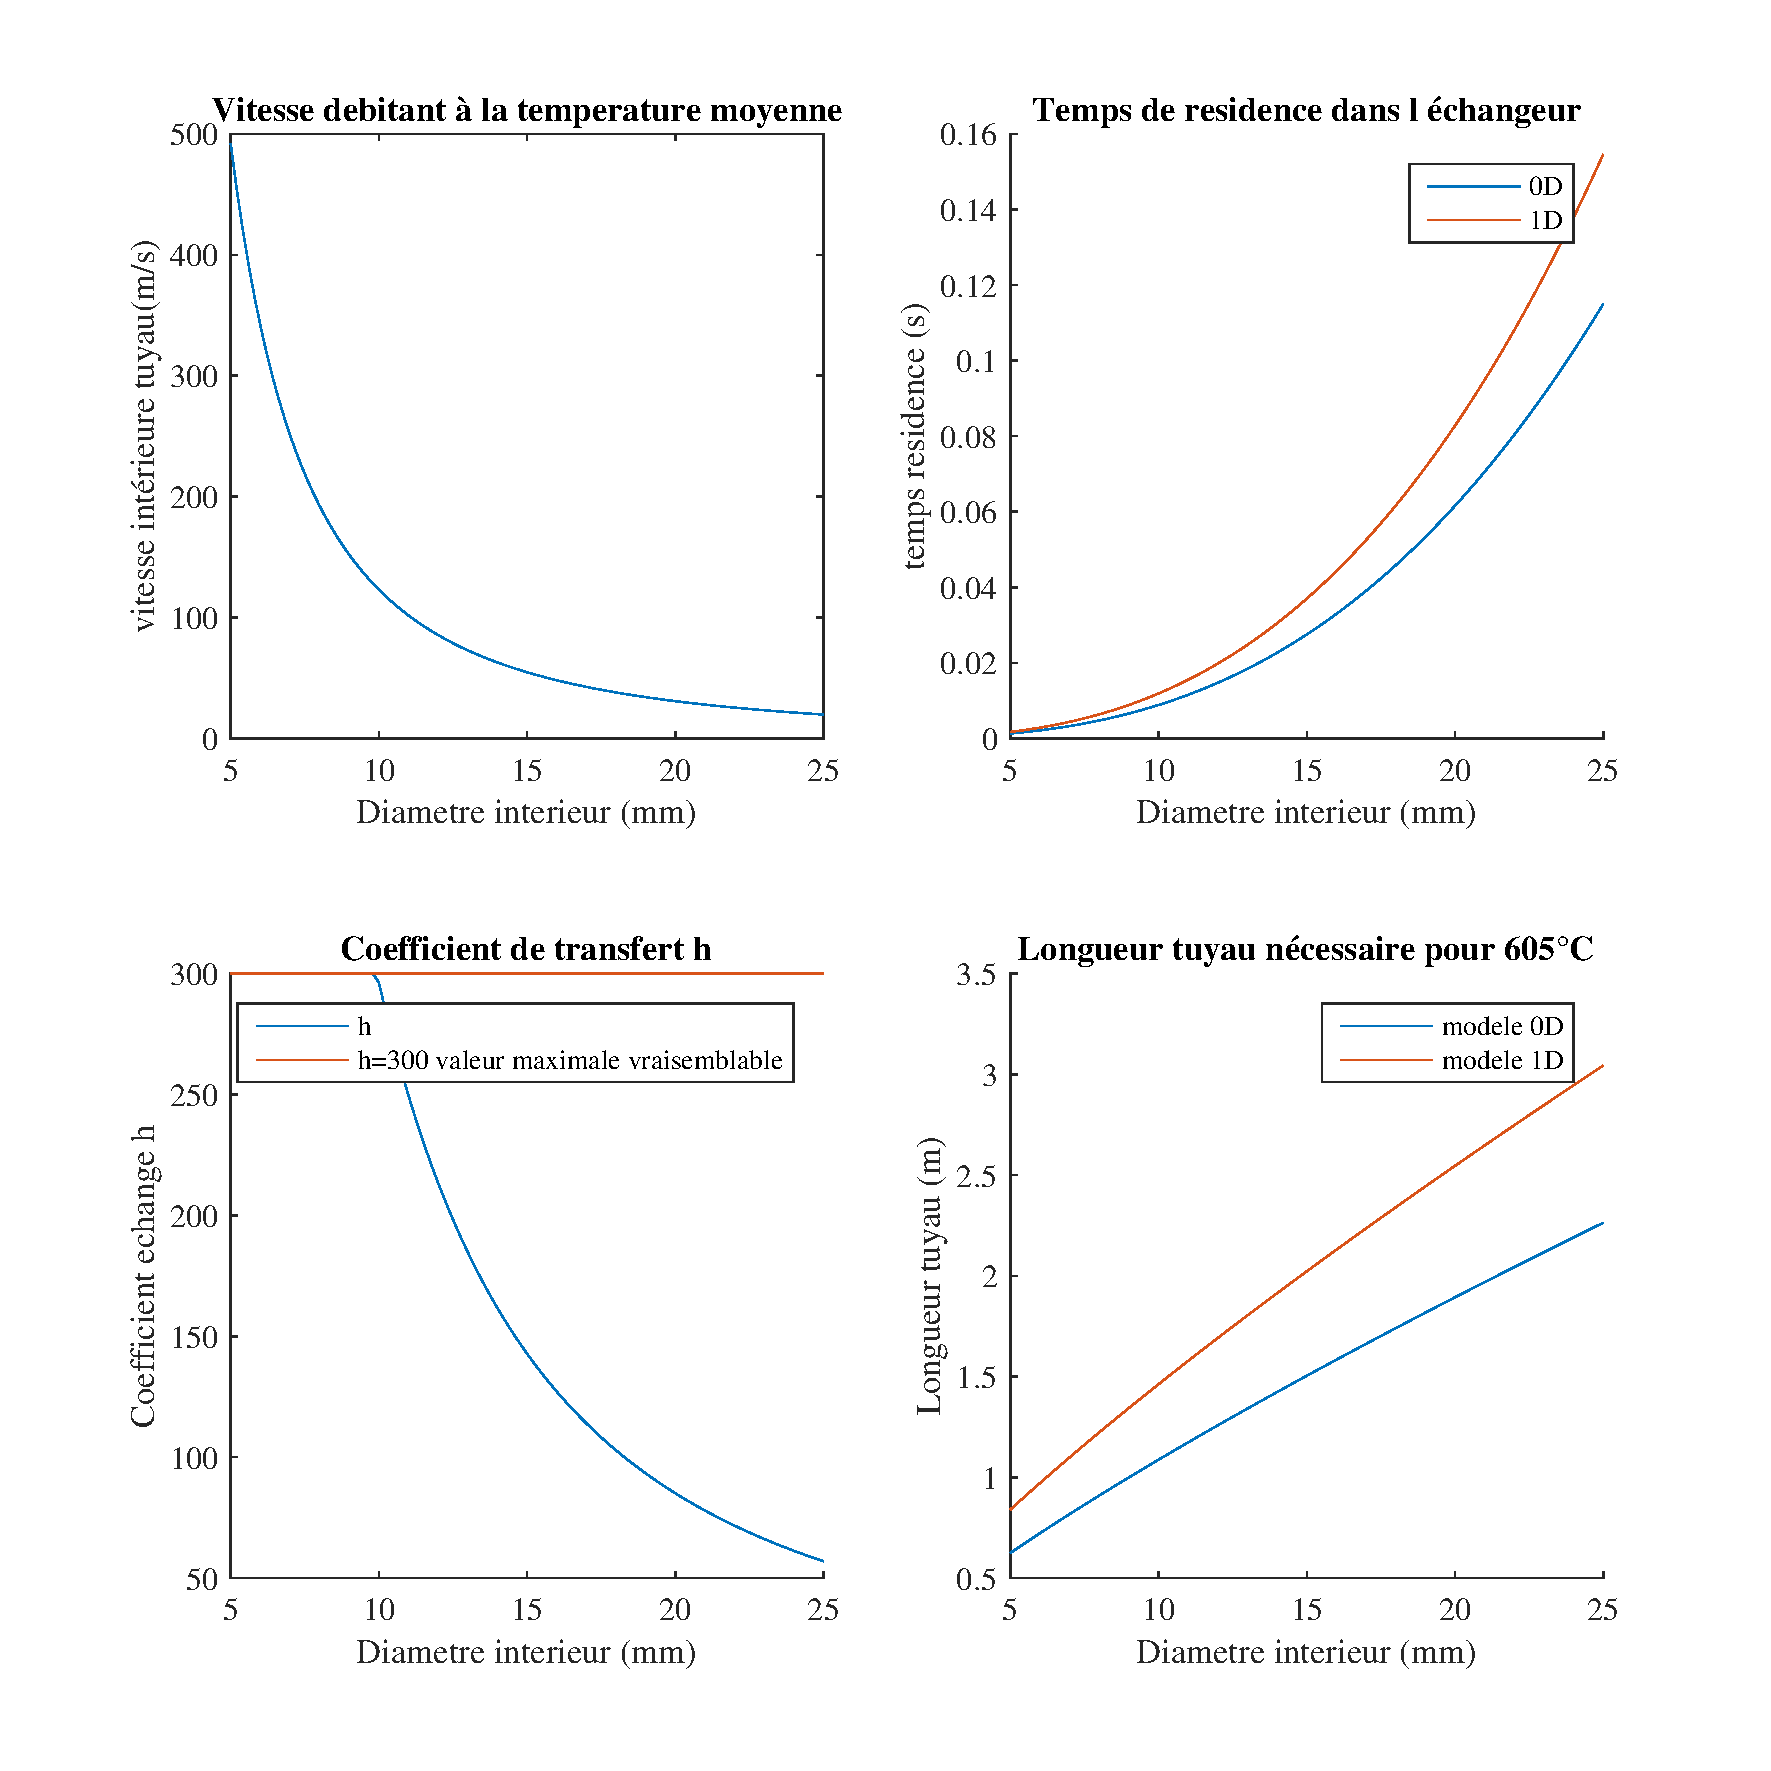
\includegraphics[width=0.9\textwidth]{fig/dimensionnement_rechauffeur.pdf}
  \caption{The heater sizing}
 \label{heater_sizing}
\end{figure}

Depending on what can be crafted, we may choose a 6meters long pipe of 20mm as internal diameter.
\renewcommand\evenpagerightmark{{\scshape\small Scale-up}}
\chapter[Scale-up]%
{Scale-up}
\label{Scale-up}

\section{The geometry}
\subsection{What is required}

The main objective of this burner is to investigate the effect of swirl on diffusion flame in an oxycombustion with a coaxial shape. The  work on ATR30 burner has been to establish an environment similar to the Freiberg OPTISOS study (in terms of flame topology ) with scale-up rules : conservation of geometry, speeds, swirl, $Z_{st}$, $J$. The aim of this burner is to be studied in a very similar environment as the study on ATR30 burner. Consequently, though the geometry is to evolve, a particular care is paid so that the speeds and the mass flows remain constant.

Let us make a bill of specifications for that burner :
\begin{enumerate}
\item The Swirl number must be modular from 0 to 2 (margins included)
\item The outlet speeds must be the same as the OPTYSOS study
\item The mass flows have to be similar to the Calhory sizing study with ATR30 burner
\item The internal axial swirled pipe will be the same as the ATR30 burner (since it is already crafted)
\item The $H_{2}O$ intermediate injection will not be used
\item The geometry must be convenient with combustion (in particular, the wall between the fuel and the oxidant must not exceed $1-2mm$, so as to prevent the flame from fixing itself in the shear stress boundary limit)  
\item The shape must be as simple as possible
\end{enumerate}
One must acknowledge that these objectives do not seem so ambitious, but the following study stresses the difficulties.

\begin{figure}[h!]
  \centering
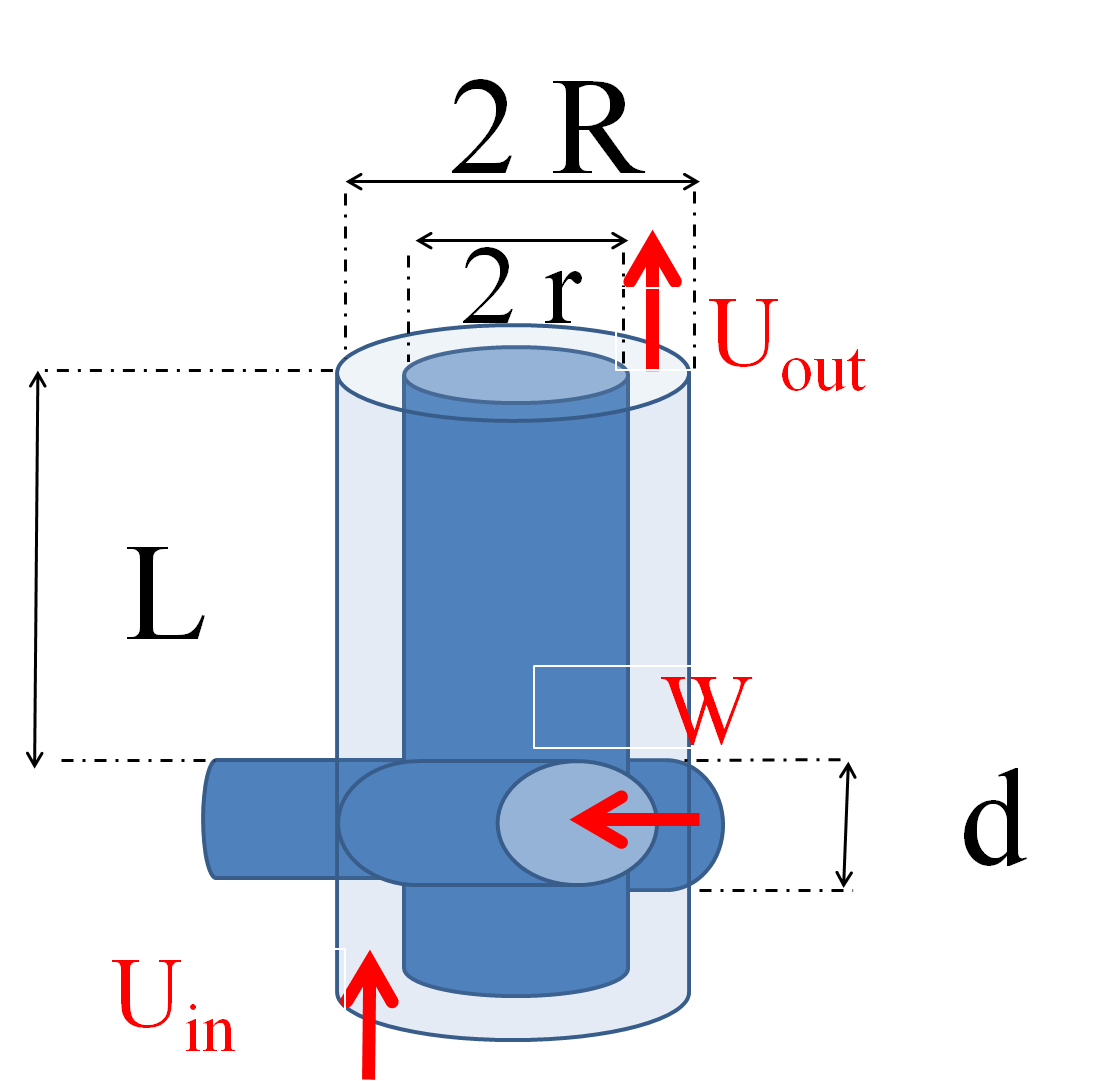
\includegraphics[width=0.50\textwidth]{fig/Proto.png}
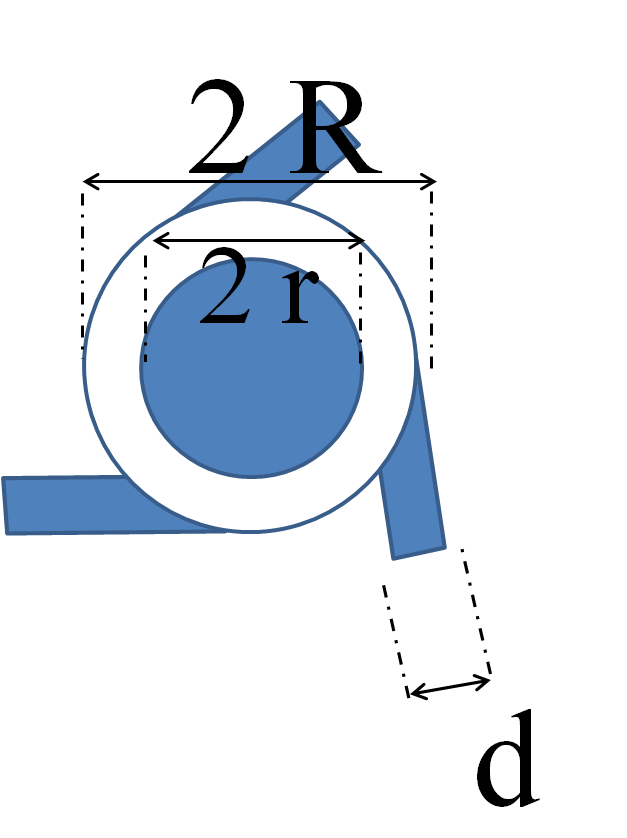
\includegraphics[width=0.40\textwidth]{fig/proto_dessus.png}
  \caption{Notations and hypothetical geometry of the prototype burner}
 \label{proto_pipe}
\end{figure}
Figure \ref{proto_pipe} gives the geometrical notations. Only the outer flow is studied, since the internal pipe is the pipe of the ATR30norm, whose geometry and swirl are already given.

Let us call $U_{out}$ the speed at the outlet of the outer pipe (at the top of the figure), $U_{in}$ the speed at the inlet of the outer pipe and $W$ the speed in the tangential pipes.

The mass conservation gives :
\begin{equation}
\dot{m_{in}}+\dot{m_{tangential}}=\dot{m_{out}}
\end{equation}


The fluid being the same in the axial and the tangential injections, we have :
\begin{equation}
U_{in}+W \frac{A_{\theta}}{A_{z}}=U_{out}
\end{equation}


\subsection{The problem of tangential speed}

In this section, it is demonstrated that the geometrical area providing the tangential injections needs to be as big as possible.

Let us consider the case where the swirl is maximum, so that the mass flow entirely comes from the tangential injections, and the injected axial flow is null. Then the mass conservation gives :
\begin{equation}
W=U_{out} \frac{A_{z}}{A_{\theta}}
\end{equation}


For practical reasons, $W$ is required smaller than $75m/s$. $U_{out}$ is the speed we want to fit to Optysos study, so it is fixed to $U_{out}=75m/s$. 

\subsection{First try with circular pipes injections}

It is demonstrated that the pipe geometry for the tangential injections seems not a good solution.

If the axial pipe goes from $r$ to $R$, there is only the room $d=R-r$ to put a circular pipe of diameter $d$ between the boundaries of the axial pipe.
If we compute the ratio :
\begin{equation}
\frac{A_{\theta}}{A_{z}}=\frac{N\pi d^2/4}{\pi (R^2-r^2)}
\end{equation} N being the number of tangential injections

Then, we  have :
\begin{equation}
 \frac{A_{\theta}}{A_{z}}=\frac{N(R-r)}{4 (R+r)}
\end{equation}

 since $r$ is fixed to $7.05mm$, we see that we need $R$ big and $N>4$  so that $W<75m/s$.
 
 This is impossible to achieve. The first conclusion is that using circular pipes for tangential injections as it is the case in fig \ref{proto_pipe} will give too big tangential speeds.
 
 \subsection{Paralepipedic injections }

Let us now consider that there are $N$ injections of paralepipedic pipes, of diameter $d$ and height $H$, as it is shown in fig \ref{proto_par}

\begin{figure}[h!]
  \centering
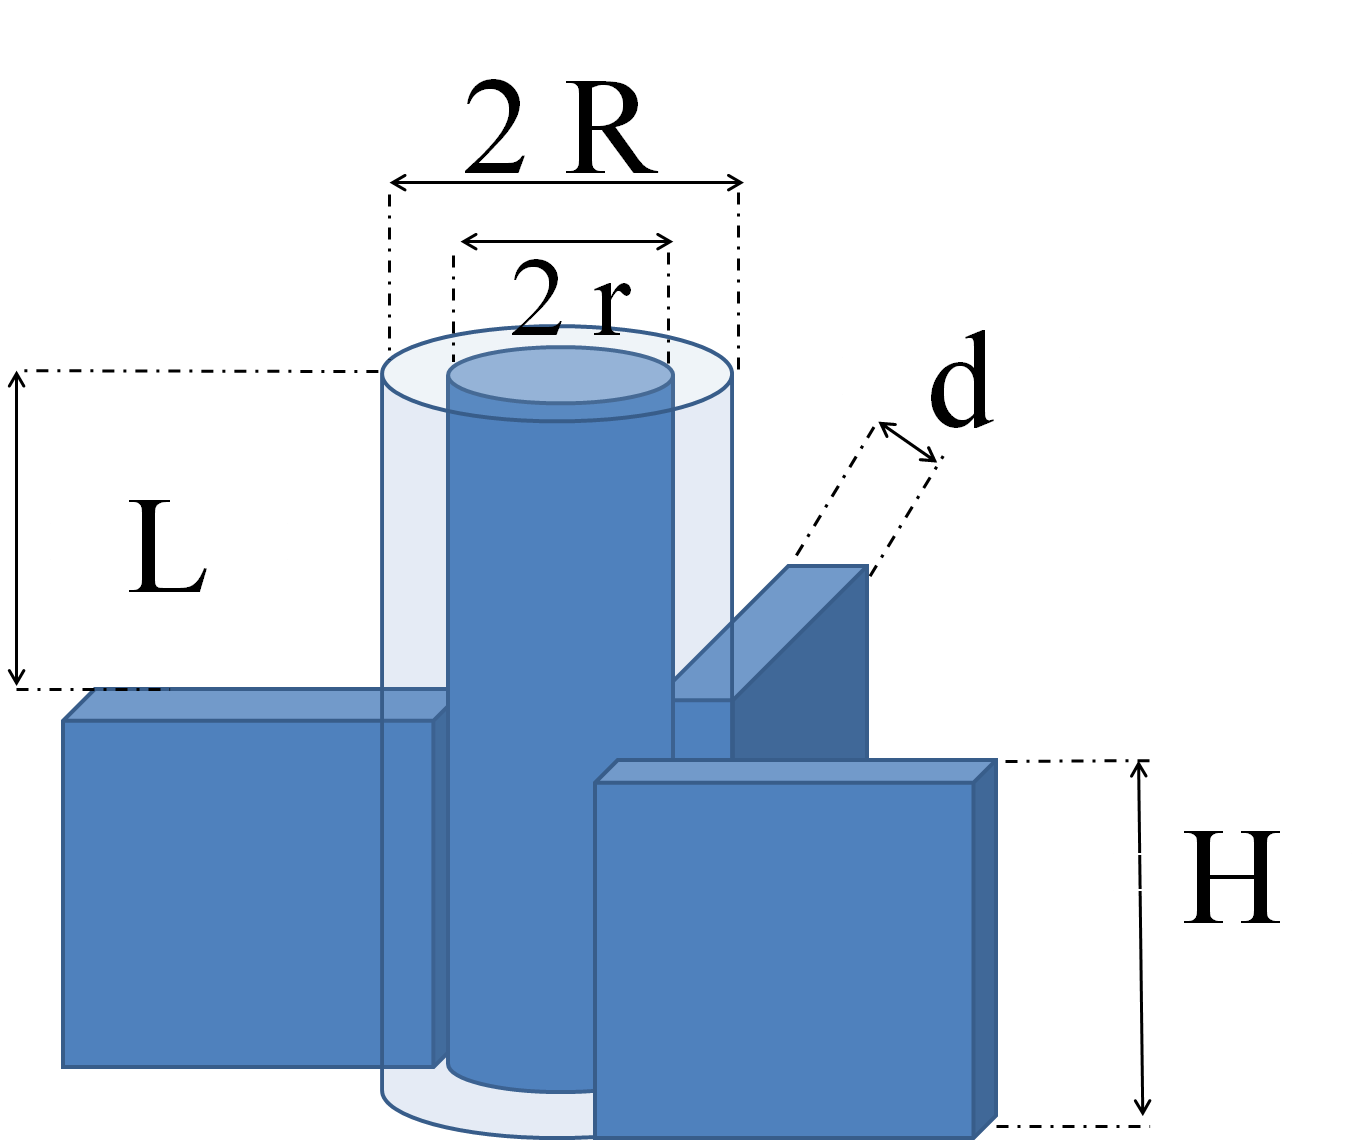
\includegraphics[width=0.45\textwidth]{fig/proto_par.png}
  \caption{Notations and hypothetical geometry of the prototype burner}
 \label{proto_par}
\end{figure}
It has been seen that $d$ must be maximized : $d=R-r$. The parameter H has now to be sized with :
\begin{equation}
W =U_{out}\frac{A_{z}}{A_{\theta}}
\end{equation}


Hence, it goes :
\begin{equation}
W=U_{out}\frac{\pi (R^2-r^2)}{NdH}
\end{equation}

Multiple tangential injections being complicated to craft, it is considered that the maximum injection number is $N=3$. In order to limit the tangential speed to 75m/s in the "worst case" (the flow is entirely tangential), we have : $H=\frac{\pi (R^2-r^2)}{Nd}=20mm$ .

Though a paralepiped injection may be harder to craft, for now it is the only investigated solution to prevent from high speeds in the burner.

\subsection{The computation of the swirl number}

The difficulties of the computation of the swirl number have previously been underlined : every mistakes or discussions starts from the assumptions on the tangential $W$ profile (constant, solid body rotation, vortex...). 

As it as been seen, in case of a swirled annular pipe, the profile $W(r)=cste \cdot \delta(r)_{r \in [R-d,R]}$ has been chosen, as it is shown in fig \ref{proto_profile}.

\begin{figure}[h!]
  \centering
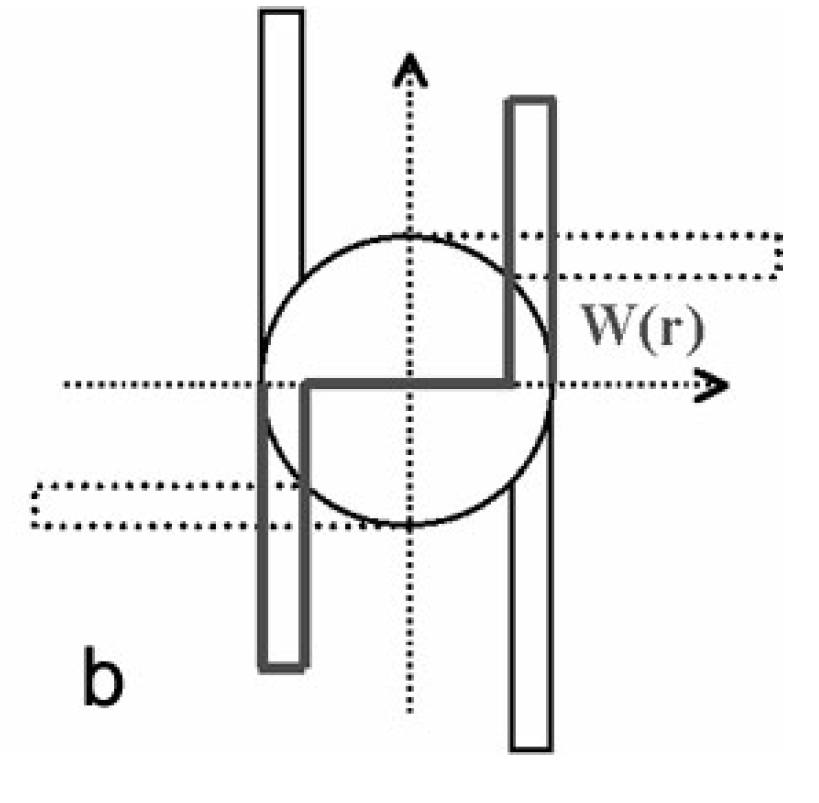
\includegraphics[width=0.45\textwidth]{fig/proto_W_profile.PNG}
  \caption{Notations on W(r) profile}
 \label{proto_profile}
\end{figure}
We thus have :
\begin{itemize}
\item from $0$ to $r$ : it is the inner pipe with axial swirl, so the speed of the outer annular pipe has no value in that area
\item from $r$ to $R-d$, we have $U_{out}=cste$ and $W(r)=0$
\item from $R-d$ to $R$, we have $U_{out}=cste$ and $W(r)=cste$
\end{itemize}



Here goes the calculations on swirl number:
\begin{equation}
S=\frac{\int_{r}^{R} W \cdot U_{out} r^2 dr}{R\int_{r}^{R}  U_{out}^2 r dr}
\end{equation}

\begin{equation}
S=\frac{W\int_{R-d}^{R} r^2dr}{R U_{out} \int_{r}^{R}  r dr}
\end{equation}

\begin{equation}\label{eq:S_proto_speed}
S=\frac{W \cdot d (R^2+d^2/3-dR)}{U_{out}R(R^2-r^2)/2}
\end{equation}
The mass conservation giving $U_{in}+W \frac{A_{\theta}}{A_{z}}=U_{out}$ , it goes in the general case (with no constraint on the shape of the tangential injection):
\begin{equation}
S=\frac{1}{1+\frac{\dot{m_{in}}}{\dot{m_{\theta}}}}\frac{A_{z}}{A_{\theta}}\frac{2d}{R}\frac{(1+\frac{d^2}{3R^2}-\frac{d}{R})}{1-(\frac{r}{R})^2}
\end{equation}


In case of a rectangular injection, here are the simplifications :
\begin{equation}
S=\frac{1}{1+\frac{\dot{m_{in}}}{\dot{m_{\theta}}}}\frac{2 \pi R}{NH}(1+\frac{d^2}{3R^2}-\frac{d}{R})
\end{equation}


To limit the speed of $W$, $A_{\theta}$ has been maximized as far as $d=R-r$.

Hence, we finally have :
\begin{equation}
S=\frac{1}{1+\frac{\dot{m_{in}}}{\dot{m_{\theta}}}}\frac{2 \pi R}{3NH}(1+\frac{r}{R}(1+\frac{r}{R}))
\end{equation}


Unfortunately, the calculation of this swirl number gives $S=0.81$, which is considered as too small : indeed, that swirl rotation can be dissipated, and let us keep in mind that this swirl is just an approximation of the real Swirl number. Many references record that the LDV-measured swirl number is two times smaller of the computed one. As a conclusion, since the internship wants to investigate large swirl number values, another design is to be found so as to reach higher predicted swirl number.

We can use the results from \ref{eq:S_proto_speed}, where the speed ratio appears :
\begin{equation}
S=\frac{W \cdot d (R^2+d^2/3-dR)}{U_{out}R(R^2-r^2)/2}
\end{equation}


To simplify it with $d=R-r$:
\begin{equation}
S=\frac{W}{U_{out}}\frac{2}{3}\frac{(1+(\frac{r}{R})^2+\frac{r}{R})}{1+\frac{r}{R}}
\end{equation}


$r$ being fixed, $R$ is plotted in figure \ref{proto_plot}. It seems there is no solution with this configuration. The need to take $\frac{W}{U_{out}}$ smaller than 1 makes the swirl very small in every configuration.


\begin{figure}[h!]
  \centering
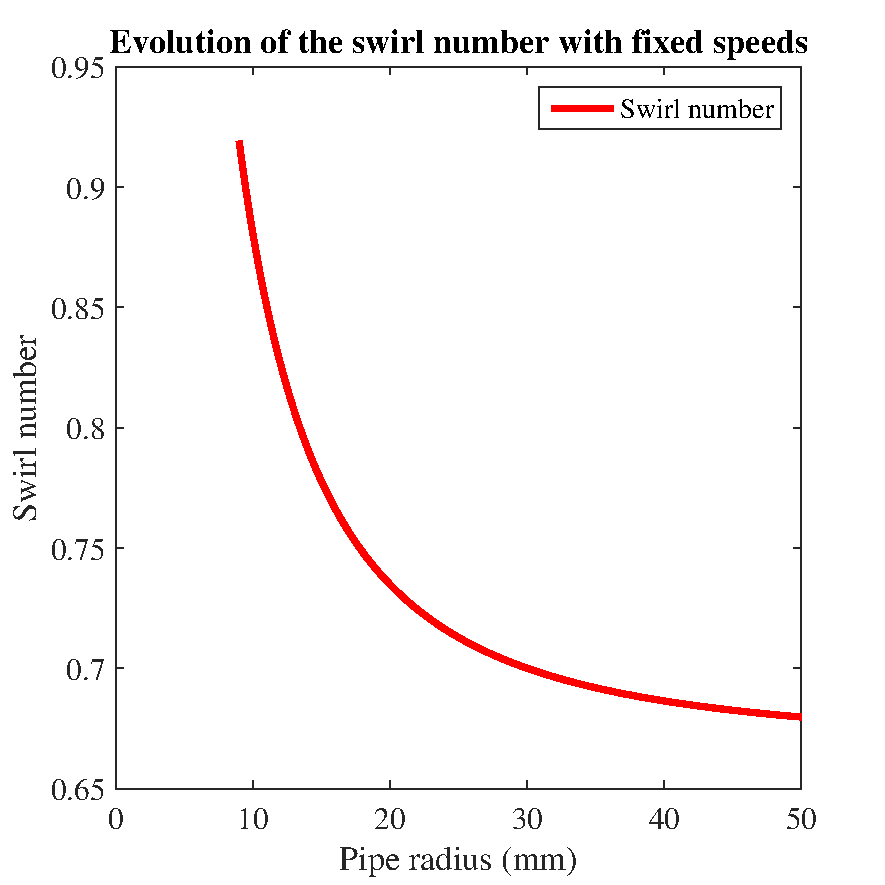
\includegraphics[width=0.7\textwidth]{fig/Proto_burner_Swirl.pdf}
  \caption{Notations on W(r) profile}
 \label{proto_plot}
\end{figure}




\renewcommand\evenpagerightmark{{\scshape\small The diffusion flame length prediction}}
\chapter[The diffusion flame length prediction]%
{The diffusion flame length prediction}
\label{The diffusion flame length prediction}
\section{An extensive review of the diffusion flame length formula }

Here is the list of all the formulas that I have found to predict a diffusion flame length. Though they seem very different, a detailed analysis will then show that they share many common features.

It is of importance to understand their origins, they can have three origins :
\begin{itemize}
\item analytical solution thanks to simplifications of the mechanisms
\item academic experiments in laboratory
\item industrial reports 
\end{itemize}

The used parameters will not be the same in the different cases, but it is very interesting to compare them.

\subsection{Laminar regime}
In a the laminar case : in (\# ref Veynante), the length of a diffusion flame in the laminar case is 
\begin{equation} \label{eq:length_laminar}
\frac{L_{f}}{e_{0}}=\frac{Re}{2\pi}\cdot \frac{1}{Z_{st}^2}
\end{equation}

  Though the regime is not of interest for industrial considerations, this formula con be demonstrated with medium effort, and permits to understand the most important parameters that drives the diffusion flame topology : the stoichiometric mixture fraction $Z_{st}$.
  \begin{equation}
Z_{st}=(1+\frac{\nu Y_{F,1}}{Y_{O_{2},2}})^{-1}
\end{equation}
  where $\nu$ is the mass stoechiometric ratio (4 for $CH_{4}-O_{2}$ flame),    $Y_{F,1}$ the mass ratio of fuel in the fuel injection ($Y_{F,1}=1$ if it is pure $CH_{4}$) and $Y_{O_{2},2}$ the mass ratio of oxygen in the oxidant injection ($Y_{O_{2},2}=0.23$ if it is pure air). One understands here that the stoichiometric mixture fraction is completely independent of the speeds, the mass flow, the bulk flow and the geometry. $Z_{st}$ only describes the composition of the gas. 

\subsection{Turbulent regime}

\subsubsection{Analysis from Peters  \cite{peters_four_1997}}
The analysis of Peters comes from the scenario of a fuel jet in a fixed oxidant :
\begin{equation}\label{eq: L_Peters}
\frac{L+x_{0}}{d}=\frac{2.19 (1+2Sc)}{Z_{st}}\frac{\rho_{0}}{\rho_{st}C}
\end{equation}

Where $Sc$  is the fixed turbulent Schmidt, $C$ the Chapman-Rubesin parameter, $\rho_{0}$ is the density at the nozzle and $\rho_{st}$ the density at the stoichiometry. $d$ is the diameter of the nozzle and $x_{0}$ the flame liftoff.

What mostly matters here is the stoichiometric mixture fraction still appears, and that $L$ depends on $\frac{1}{Z_{st}}$ in the turbulent case instead of $\frac{1}{Z_{st}^2}$ as it is the case in laminar regime.

It will be seen that this dependency on $\frac{1}{Z_{st}}$ is the characteristic of a diffusion turbulent flame.

\subsubsection{Experiment from Hawthorne \cite{hawthorne_mixing_????}}



Hawthorne gets experimentally the length  :
\begin{equation}\label{eq :L_hawthorne}
\frac{L+x_{0}}{d}=\frac{5.3}{Z_{st}}(\frac{\rho_{0}}{\rho_{st}})^{-1/2}
\end{equation}
Since it is quite close to Peters analysis \ref{eq: L_Peters}, Peters chose to fix in his formula $Sc$ and $C$ in order to fit to Hawthorne formula.

\paragraph{Numerical application} For a methane/air flame, we have $Z_{st}=(1+4\frac{1}{0.233})^{-1}=0.055$. Assuming $T_{st}=2000K$, it goes $\frac{\rho_{0}}{\rho_{st}}\sim 3.8$ and $L \sim 200d$.


\subsubsection{IFRF Online Combustion Handbook (industrial formula)\cite{neil_fricker_ifrf_2001}}

Here is the length $x_{s}$ where a jet can reach the stoichiometric equilibrium without combustion. We are now in an industrial case and not in the academic area :

\begin{equation}
x_{s}=5.9\Phi (1+\frac{V_{a}}{d_{g}})
\end{equation} with $\Phi=2\frac{Q_{m}}{\sqrt[]{\pi G \rho_{f}}}$. It can be noted that the notations are much more "industrial" :
\begin{itemize}
\item $V_{a}$ is "Stoichiometric Air Requirement (or Air Requirement) - The quantity of air required to completely combust a given quantity of a fuel - may be expressed on a volume or a mass or a mixed volume/mass basis (Vol/Vol)"
\item $d_{g}$ is the specific gravity of the fuel (density with respect to air)
\item $Q_{m}$ is the mass flow of fuel gas (kg/s)
\item $\rho_{f}$ is the density of the combustion products in the flame (kg/m3)
\item $G$ is the thrust of the incoming fuel jet (N)
\end{itemize}

It seems that this formula is completely new uncorrelated from the previous ones, however, using :
$Q_{air}\rho_{air}= \dot{m}_{air}$ and $Q_{fuel}\rho_{fuel}= \dot{m}_{fuel}$  ($Q$ being the bulk flow), we get :

\begin{equation}
V_{a}=\frac{Q_{air}}{Q_{fuel}}=\frac{ \dot{m}_{air}}{ \dot{m}_{fuel}}d_{g}
\end{equation}
Hence, using $\dot{m}_{CH_{4}}=Y_{1,CH_{4}}\cdot \dot{m}_{fuel}$and $\dot{m}_{O_{2}}=Y_{2,O_{2}}\cdot \dot{m}_{air}$
\begin{equation}
1+\frac{V_{a}}{d_{g}}=1+\frac{ \dot{m}_{air}}{ \dot{m}_{fuel}}=1+\frac{\nu Y_{F,1}}{Y_{O_{2},2}}=\frac{1}{Z_{st}}
\end{equation}

Consequently, it has been found that the industrial flame length formula also depends on $\frac{1}{Z_{st}}$ .

Using :
\begin{itemize}
\item $G=\dot m_{fuel} v_{fuel}$
\item $\dot m_{fuel}= v_{fuel} \cdot S_{fuel} \cdot \rho_{fresh fuel}$
\end{itemize}

And making the correspondence between the industrial and academic notations :
\begin{itemize}
\item $\rho_{fresh fuel}= \rho_{0} $
\item $\rho_{f}=\rho_{st}$
\item $Q_{m}=\dot{m}_{fuel}$
\end{itemize}
It goes :

\begin{equation}
\frac{x_{s}}{d}=5.92\frac{2Q_{m}}{\sqrt[]{\pi G \rho_{f}}}\frac{1}{Z_{st}}=\frac{5.92}{Z_{st}}(\frac{\rho_{0}}{\rho_{st}})^{1/2}
\end{equation} 
The formula is exactly the same as the one of Peters, except the factor.

The purpose of these formulas is obviously not to use them for a much more complicated case (swirled coaxial flow), but to consider that all the parametric parameters studied in Optisos report can be gathered with adimensional number. If these formula were correct, the flame length should depend on the stoichiometric mixture fraction $Z_{st}$, since $Z_{st}$ keeps all the information of S/C dilution, burner load or pressure variation of density.

\section{Investigation on Optisos analysis }

\subsection{Context of the investigation}

Given the lack of experimental data, predicting the flame length of the ATR burner seems is very unreachable. The experiments on Freiberg HP-POX burner are almost our only contact with industrial real results of combustion process in ATR burner. Furthermore, a detailed campaign has been made with parametric studies of different inputs, such as the S/C ratio, the load variation or the Oxygen/NG velocity ratio. The chosen metric to investigate the flame topology here will be the flame length 

The conclusion of the report are that :
\begin{enumerate}
\item Changing the pressure of the ATR burner from 30 to 50 bars leads to small variation of the flame length
\item The S/C ratio is the parameter that the biggest impact on the flame topology : With a S/C ratio increasing from 1 to 1.4, the flame length decreases from 124mm to 84mm
\item The burner load also drives the flame length : increasing burner load shortens the flame
\item High temperatures of the reactor leads to longer flame
\end{enumerate}

In order to emphasize the conclusion of the reports, here are the corresponding plot from Optisos report :

\begin{figure}[h!]
  \centering
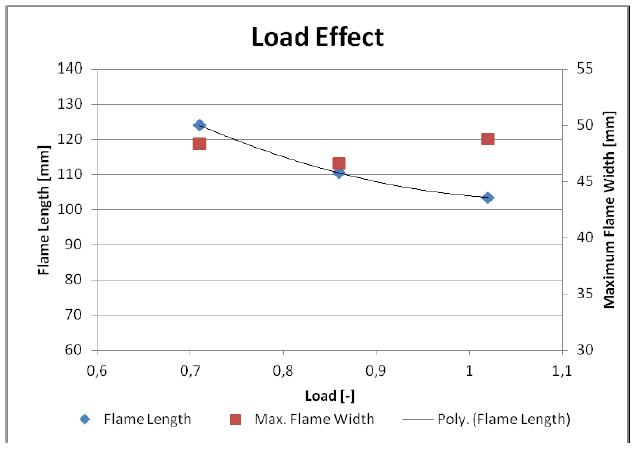
\includegraphics[width=0.45\textwidth]{fig/Optisos_Load_effect.PNG}
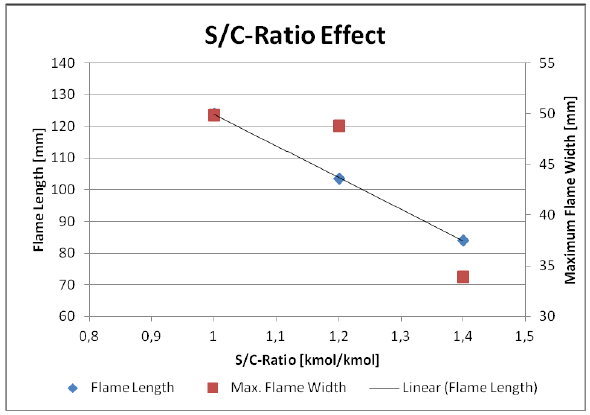
\includegraphics[width=0.45\textwidth]{fig/Optisos_S_C_effect.PNG}
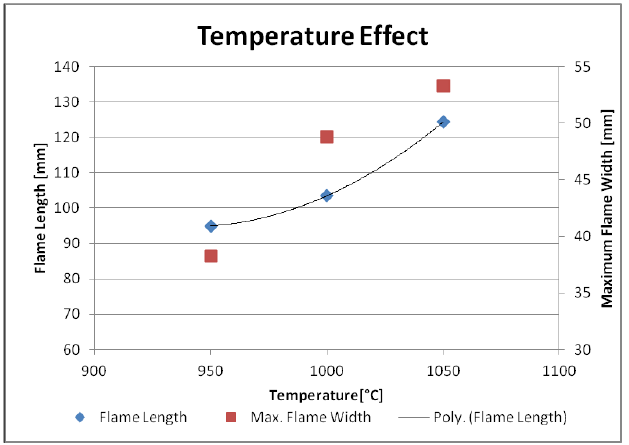
\includegraphics[width=0.45\textwidth]{fig/Optisos_temperature_effect.PNG}
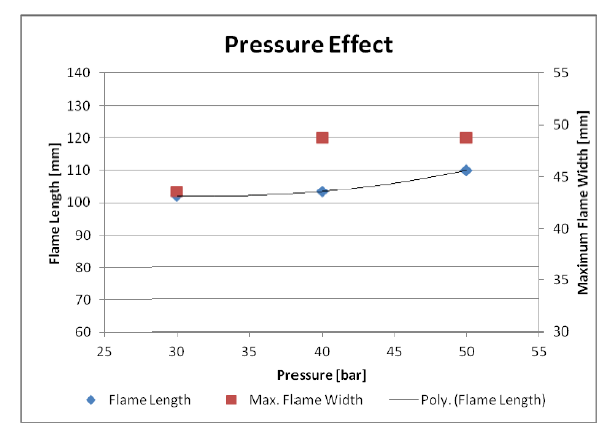
\includegraphics[width=0.45\textwidth]{fig/Optisos_Pressure_effect.PNG}
  \caption{Conclusion of Optisos report on flame topology}
 \label{optisos_plot}
\end{figure}

Dealing with my internship, if the flame length depended on so many parameters, it mean that I would have to study them all, and to keep them constant in Calhory burner with scales-up rule. This task seems impossible to achieve. Besides, a analysis of  the literature gives another interpretation. 



In this chapter, the data from Optisos has been re-used to compute in each test the corresponding $Z_{st}$, and it has be found that, in the area of the tests that have been conducted, the flame length of ATR burner measured in Optisos diagnostic directly depends on the stoichiometric mixture fraction $Z_st$ as an affine function :

The points in red are the cases where the temperature of the reactor has been changed, which does not implicate the $Z_{st}$, and adresses heat transfer and kinetic.

\begin{figure}[h!]
  \centering
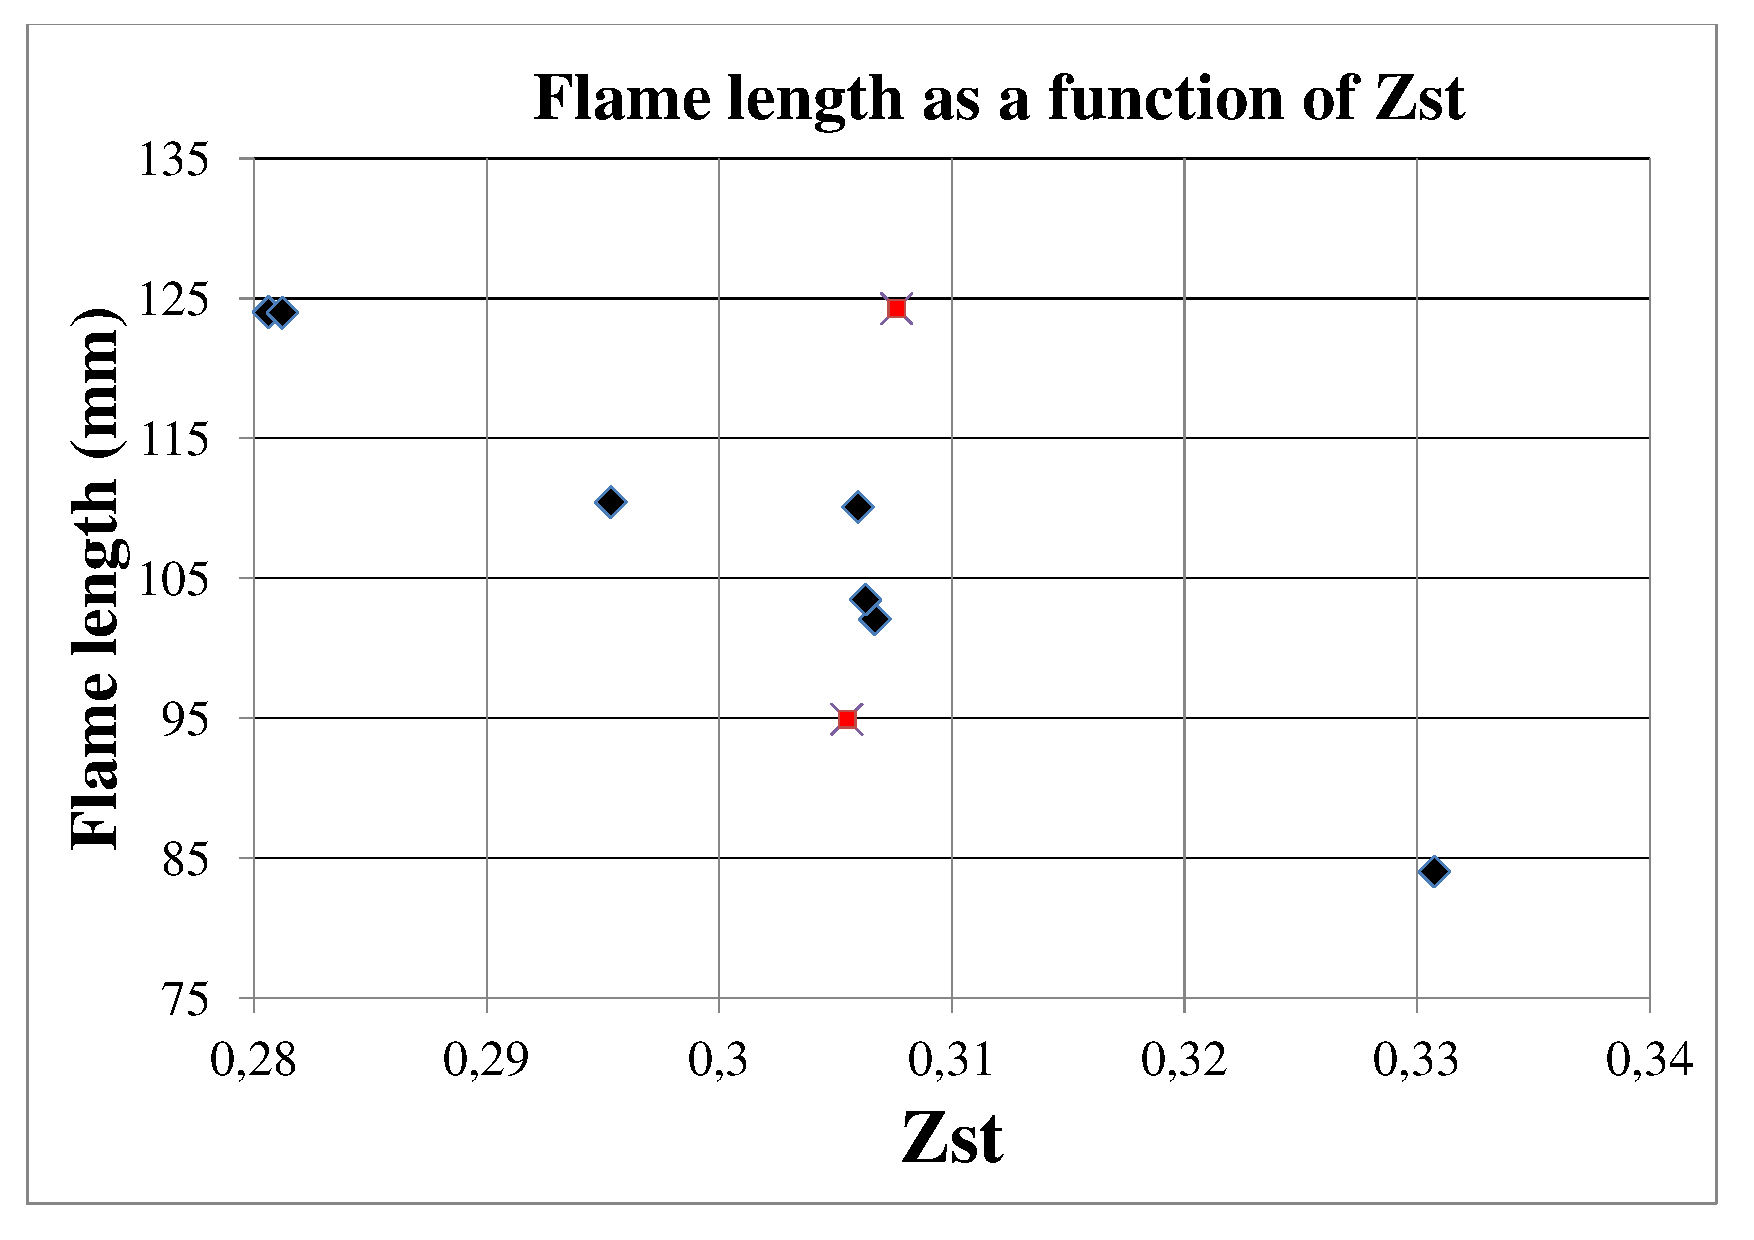
\includegraphics[width=0.8\textwidth]{fig/Flame_length_Zst.pdf}
 \label{Flame length as a function of Zst}
\end{figure}

It would be interested to get more points, or to extend the investigation segment, to define a characteristic law such as $Length=A_{0}-A_{1}\cdot Z_{st}$. One can easily verify that the trend is logical according to what have been observed previously, 

\appendix
\chapter[Protocole interférométrie différentielle ]%
{Protocole interférométrie différentielle}


\section{Principe de la mesure}

Le dispositif d'interférométrie différentielle mesure des différences de densités entre des milieux. On veut observer le profil en sortie du brûleur ATR30norm.

Ce qu'on veut observer :
\begin{itemize}
\item l'angle d'ouverture du cône
\item éventuellement la zone de mélange
\item éventuellement la présence de recirculation
\item éventuellement l'instensité de la turbulence
\end{itemize}

\section{Ecoulement d'air}
Il s'agira uniquement d'air, chauffé entre $20^\circ C$ et $600^\circ C$, au moyen d'un four et d'un échangeur placé à l'intérieur. Le four peut atteindre la température de $850^\circ C$ , les calculs de l'échangeurs ont été faits pour que l'air en sortie atteigne $600 ^\circ C$. On ajustera la consigne du four pour que le thermocouple de l'air chaud indique la température désirée.

Il est à noter que la précision recherchée pour la température n'est pas très exigeante ($ > 20^\circ C$).
\begin{figure}[!h]
  \centering
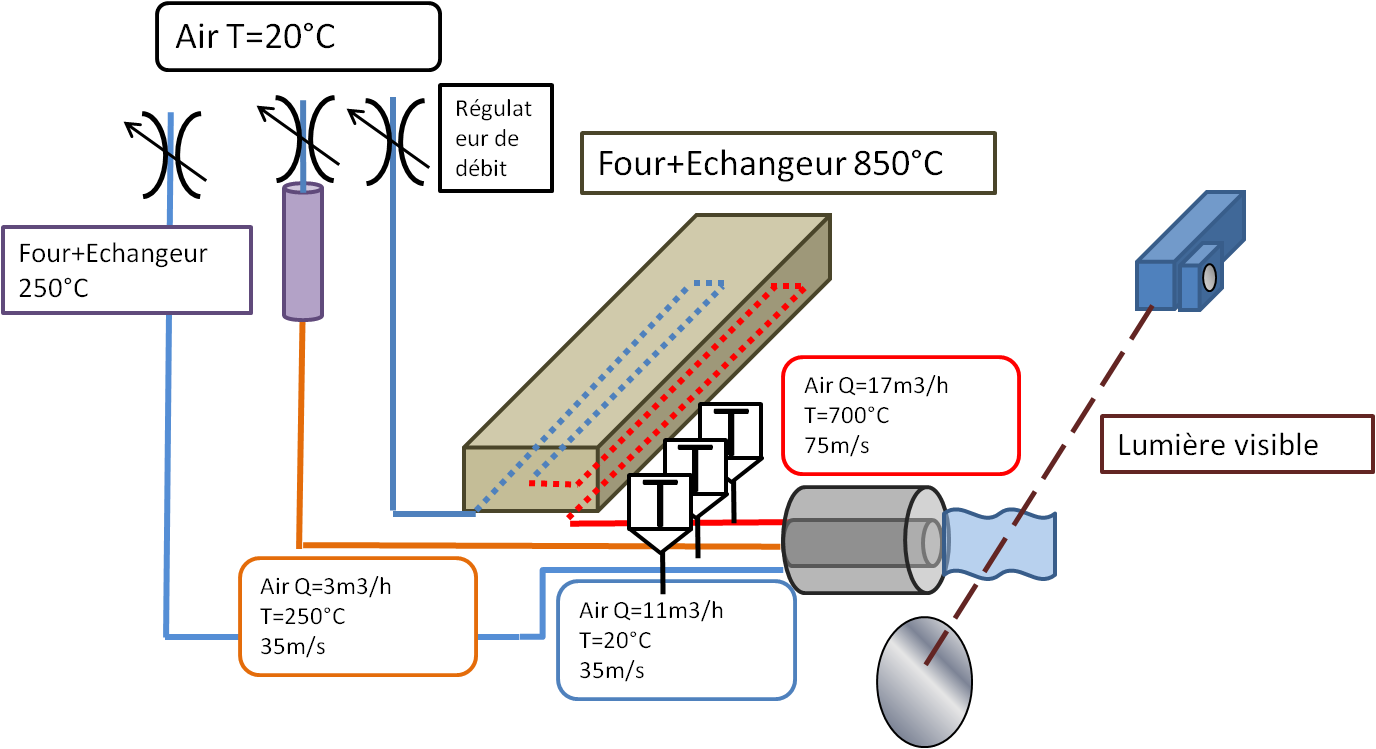
\includegraphics[width=0.8\textwidth]{fig/EPR_schema_installation.png}
  \caption{Schema de l'installation}
 \label{schema_installation}
\end{figure}

\begin{figure}[!h]
  \centering
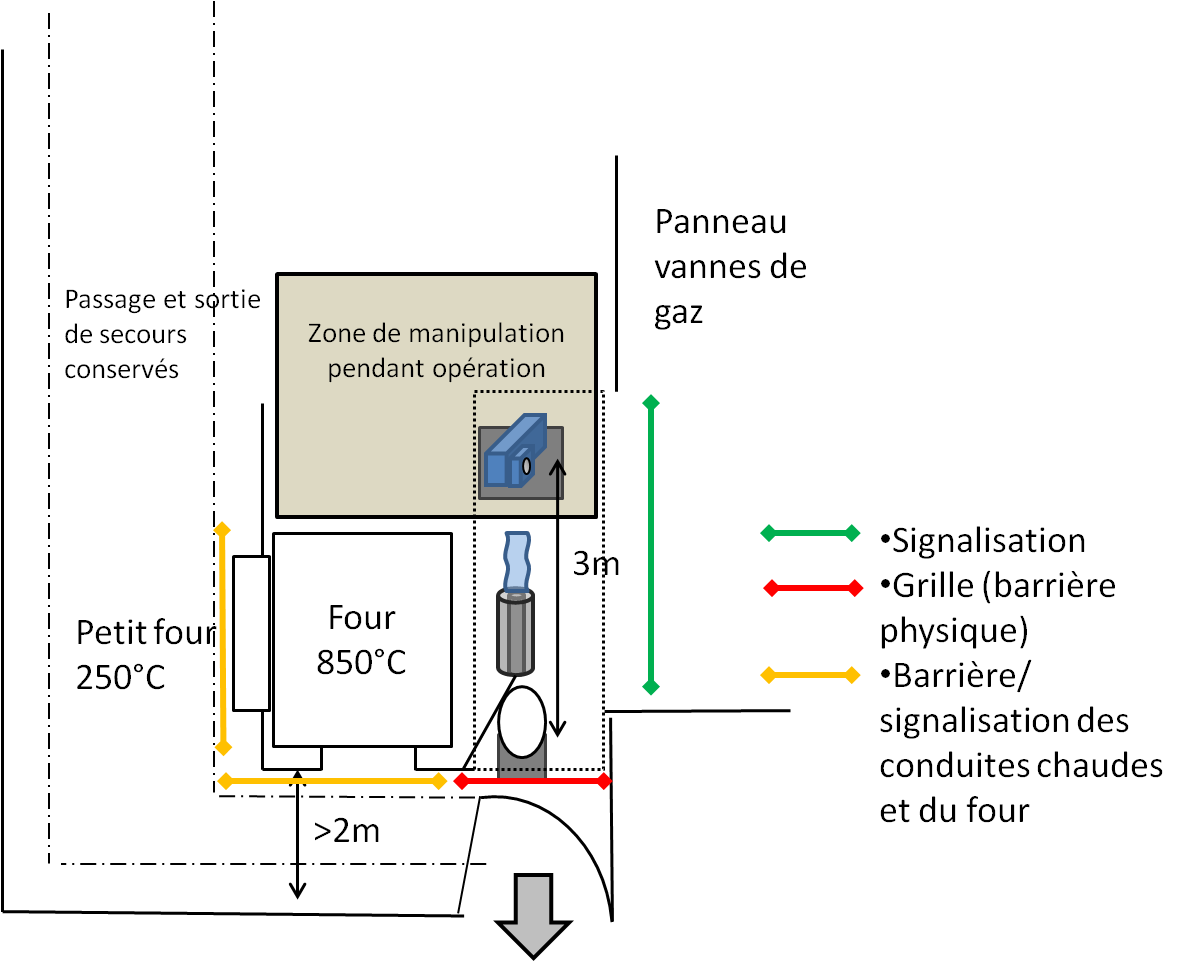
\includegraphics[width=0.8\textwidth]{fig/EPR_plan_de_travail.png}
  \caption{Plan de travail}
 \label{plan_travail}
\end{figure}
\newpage
\section{Plan de la manipulation}
\begin{enumerate}
\item Préparation
\begin{enumerate}
\item Disposition du matériel et raccordement à froid des trois arrivées d’air
\item Vérification de l'étanchéité
\item Réchauffeur placé dans le four
\item Four en position « pseudo-fermée » (25mm d’espace encore ouvert avant la butée)
\item Calorifugeage du four et des conduites d’air chaud
\item Calibration et focus du système optique sans écoulement
\item Changement de la consigne de sécurité du four pour que le four puisse démarrer en position « pseudo-fermée »
\item Balisage et pose des barrières de sécurité
\end{enumerate}
\item Mise en route
\begin{enumerate}
\item Chauffage des fours
\item Mise en écoulement de l’air
\item Asservissement de la température du four selon la consigne $T=600 ^\circ C$  pour l’air chaud
\end{enumerate}
\item Diagnostic/Mesures
\begin{enumerate}
\item Le diagnostic, les manipulations et ses éventuelles corrections optiques se font au minimum à une distance de deux mètres de l’écoulement
 \end{enumerate}
\item Fin de manipulation
\begin{enumerate}
\item Fermeture des débits d’air
\item Coupure des fours
\item Attente que le dispositif se refroidisse
 \end{enumerate}
\item Post Manipulation
\begin{enumerate}
\item Rétablir le seuil de sécurité d’origine du four (sécurité en butée : four fermé)
\item Etablir le procès verbal de fin d’opération
 \end{enumerate}
 \end{enumerate}
\section{Précautions particulières}
 On fera attention à :
 
 \begin{itemize}
\item Choisir des supports très stables pour le dispositif optique ainsi que le support du brûleur
\item Protéger la caméra rapide
\item L'écoulement d'air sera très bruyant, prévoir des protections
\end{itemize}










%\addcontentsline{toc}{section}{}


\bibliographystyle{plain}
\bibliography{Zoterobib3.bib}

\end{document}